\documentclass{article}
\usepackage[final]{neurips_2025}  % NEURIPS style (neurips_2025.sty is in paper_draft/)
\makeatletter\providecommand{\@trackname}{\@neuripsordinal\ Conference on Neural Information Processing Systems (NeurIPS \@neuripsyear).}\makeatother
\usepackage[utf8]{inputenc}
\usepackage[T1]{fontenc}
\usepackage[hidelinks]{hyperref}  % REQUIRED: clickable links
\usepackage{booktabs}  % REQUIRED: professional tables
\usepackage{graphicx}
\usepackage{amsmath,amssymb}
\usepackage{multirow}
\usepackage{enumitem}
\usepackage{subcaption}
\usepackage{algorithm}
\usepackage[noend]{algpseudocode}

% Import command files
%%%%% MATH NOTATION MACROS %%%%%
% Standard math notation for academic papers
% Import with: %%%%% MATH NOTATION MACROS %%%%%
% Standard math notation for academic papers
% Import with: %%%%% MATH NOTATION MACROS %%%%%
% Standard math notation for academic papers
% Import with: \input{commands/math}

\usepackage{amsmath,amsfonts,bm}

%%%%%%%%%%%%%%%%%%%%%%%%%%%%%%%%%%%%%%%%%%%%%%%%%%%%%%%%%%%%%%%%%
% FIGURE AND SECTION REFERENCES
%%%%%%%%%%%%%%%%%%%%%%%%%%%%%%%%%%%%%%%%%%%%%%%%%%%%%%%%%%%%%%%%%

% Mark sections of captions for referring to divisions of figures
\newcommand{\figleft}{{\em (Left)}}
\newcommand{\figcenter}{{\em (Center)}}
\newcommand{\figright}{{\em (Right)}}
\newcommand{\figtop}{{\em (Top)}}
\newcommand{\figbottom}{{\em (Bottom)}}
\newcommand{\captiona}{{\em (a)}}
\newcommand{\captionb}{{\em (b)}}
\newcommand{\captionc}{{\em (c)}}
\newcommand{\captiond}{{\em (d)}}

% Figure references
\def\figref#1{figure~\ref{#1}}
\def\Figref#1{Figure~\ref{#1}}
\def\twofigref#1#2{figures \ref{#1} and \ref{#2}}
\def\quadfigref#1#2#3#4{figures \ref{#1}, \ref{#2}, \ref{#3} and \ref{#4}}

% Section references
\def\secref#1{section~\ref{#1}}
\def\Secref#1{Section~\ref{#1}}
\def\twosecrefs#1#2{sections \ref{#1} and \ref{#2}}
\def\secrefs#1#2#3{sections \ref{#1}, \ref{#2} and \ref{#3}}

% Equation references
\def\eqref#1{equation~\ref{#1}}
\def\Eqref#1{Equation~\ref{#1}}
\def\plaineqref#1{\ref{#1}}

% Algorithm references
\def\algref#1{algorithm~\ref{#1}}
\def\Algref#1{Algorithm~\ref{#1}}
\def\twoalgref#1#2{algorithms \ref{#1} and \ref{#2}}
\def\Twoalgref#1#2{Algorithms \ref{#1} and \ref{#2}}

% Table references
\def\tabref#1{table~\ref{#1}}
\def\Tabref#1{Table~\ref{#1}}

% Chapter references
\def\chapref#1{chapter~\ref{#1}}
\def\Chapref#1{Chapter~\ref{#1}}

%%%%%%%%%%%%%%%%%%%%%%%%%%%%%%%%%%%%%%%%%%%%%%%%%%%%%%%%%%%%%%%%%
% BASIC MATH DEFINITIONS
%%%%%%%%%%%%%%%%%%%%%%%%%%%%%%%%%%%%%%%%%%%%%%%%%%%%%%%%%%%%%%%%%

\def\ceil#1{\lceil #1 \rceil}
\def\floor#1{\lfloor #1 \rfloor}
\def\1{\bm{1}}
\def\eps{{\epsilon}}

% Common operators
\DeclareMathOperator*{\argmax}{arg\,max}
\DeclareMathOperator*{\argmin}{arg\,min}
\DeclareMathOperator{\sign}{sign}
\DeclareMathOperator{\Tr}{Tr}
\let\ab\allowbreak

%%%%%%%%%%%%%%%%%%%%%%%%%%%%%%%%%%%%%%%%%%%%%%%%%%%%%%%%%%%%%%%%%
% VECTORS (lowercase bold)
%%%%%%%%%%%%%%%%%%%%%%%%%%%%%%%%%%%%%%%%%%%%%%%%%%%%%%%%%%%%%%%%%

\def\vzero{{\bm{0}}}
\def\vone{{\bm{1}}}
\def\vmu{{\bm{\mu}}}
\def\vtheta{{\bm{\theta}}}
\def\va{{\bm{a}}}
\def\vb{{\bm{b}}}
\def\vc{{\bm{c}}}
\def\vd{{\bm{d}}}
\def\ve{{\bm{e}}}
\def\vf{{\bm{f}}}
\def\vg{{\bm{g}}}
\def\vh{{\bm{h}}}
\def\vi{{\bm{i}}}
\def\vj{{\bm{j}}}
\def\vk{{\bm{k}}}
\def\vl{{\bm{l}}}
\def\vm{{\bm{m}}}
\def\vn{{\bm{n}}}
\def\vo{{\bm{o}}}
\def\vp{{\bm{p}}}
\def\vq{{\bm{q}}}
\def\vr{{\bm{r}}}
\def\vs{{\bm{s}}}
\def\vt{{\bm{t}}}
\def\vu{{\bm{u}}}
\def\vv{{\bm{v}}}
\def\vw{{\bm{w}}}
\def\vx{{\bm{x}}}
\def\vy{{\bm{y}}}
\def\vz{{\bm{z}}}

%%%%%%%%%%%%%%%%%%%%%%%%%%%%%%%%%%%%%%%%%%%%%%%%%%%%%%%%%%%%%%%%%
% MATRICES (uppercase bold)
%%%%%%%%%%%%%%%%%%%%%%%%%%%%%%%%%%%%%%%%%%%%%%%%%%%%%%%%%%%%%%%%%

\def\mA{{\bm{A}}}
\def\mB{{\bm{B}}}
\def\mC{{\bm{C}}}
\def\mD{{\bm{D}}}
\def\mE{{\bm{E}}}
\def\mF{{\bm{F}}}
\def\mG{{\bm{G}}}
\def\mH{{\bm{H}}}
\def\mI{{\bm{I}}}
\def\mJ{{\bm{J}}}
\def\mK{{\bm{K}}}
\def\mL{{\bm{L}}}
\def\mM{{\bm{M}}}
\def\mN{{\bm{N}}}
\def\mO{{\bm{O}}}
\def\mP{{\bm{P}}}
\def\mQ{{\bm{Q}}}
\def\mR{{\bm{R}}}
\def\mS{{\bm{S}}}
\def\mT{{\bm{T}}}
\def\mU{{\bm{U}}}
\def\mV{{\bm{V}}}
\def\mW{{\bm{W}}}
\def\mX{{\bm{X}}}
\def\mY{{\bm{Y}}}
\def\mZ{{\bm{Z}}}
\def\mBeta{{\bm{\beta}}}
\def\mPhi{{\bm{\Phi}}}
\def\mLambda{{\bm{\Lambda}}}
\def\mSigma{{\bm{\Sigma}}}

%%%%%%%%%%%%%%%%%%%%%%%%%%%%%%%%%%%%%%%%%%%%%%%%%%%%%%%%%%%%%%%%%
% CALLIGRAPHIC (mathcal)
%%%%%%%%%%%%%%%%%%%%%%%%%%%%%%%%%%%%%%%%%%%%%%%%%%%%%%%%%%%%%%%%%

\def\gA{{\mathcal{A}}}
\def\gB{{\mathcal{B}}}
\def\gC{{\mathcal{C}}}
\def\gD{{\mathcal{D}}}
\def\gE{{\mathcal{E}}}
\def\gF{{\mathcal{F}}}
\def\gG{{\mathcal{G}}}
\def\gH{{\mathcal{H}}}
\def\gI{{\mathcal{I}}}
\def\gJ{{\mathcal{J}}}
\def\gK{{\mathcal{K}}}
\def\gL{{\mathcal{L}}}
\def\gM{{\mathcal{M}}}
\def\gN{{\mathcal{N}}}
\def\gO{{\mathcal{O}}}
\def\gP{{\mathcal{P}}}
\def\gQ{{\mathcal{Q}}}
\def\gR{{\mathcal{R}}}
\def\gS{{\mathcal{S}}}
\def\gT{{\mathcal{T}}}
\def\gU{{\mathcal{U}}}
\def\gV{{\mathcal{V}}}
\def\gW{{\mathcal{W}}}
\def\gX{{\mathcal{X}}}
\def\gY{{\mathcal{Y}}}
\def\gZ{{\mathcal{Z}}}

%%%%%%%%%%%%%%%%%%%%%%%%%%%%%%%%%%%%%%%%%%%%%%%%%%%%%%%%%%%%%%%%%
% SETS (blackboard bold)
%%%%%%%%%%%%%%%%%%%%%%%%%%%%%%%%%%%%%%%%%%%%%%%%%%%%%%%%%%%%%%%%%

\def\sA{{\mathbb{A}}}
\def\sB{{\mathbb{B}}}
\def\sC{{\mathbb{C}}}
\def\sD{{\mathbb{D}}}
\def\sF{{\mathbb{F}}}
\def\sG{{\mathbb{G}}}
\def\sH{{\mathbb{H}}}
\def\sI{{\mathbb{I}}}
\def\sJ{{\mathbb{J}}}
\def\sK{{\mathbb{K}}}
\def\sL{{\mathbb{L}}}
\def\sM{{\mathbb{M}}}
\def\sN{{\mathbb{N}}}
\def\sO{{\mathbb{O}}}
\def\sP{{\mathbb{P}}}
\def\sQ{{\mathbb{Q}}}
\def\sR{{\mathbb{R}}}
\def\sS{{\mathbb{S}}}
\def\sT{{\mathbb{T}}}
\def\sU{{\mathbb{U}}}
\def\sV{{\mathbb{V}}}
\def\sW{{\mathbb{W}}}
\def\sX{{\mathbb{X}}}
\def\sY{{\mathbb{Y}}}
\def\sZ{{\mathbb{Z}}}

%%%%%%%%%%%%%%%%%%%%%%%%%%%%%%%%%%%%%%%%%%%%%%%%%%%%%%%%%%%%%%%%%
% COMMON MATH SHORTCUTS
%%%%%%%%%%%%%%%%%%%%%%%%%%%%%%%%%%%%%%%%%%%%%%%%%%%%%%%%%%%%%%%%%

% Expectation and variance
\newcommand{\E}{\mathbb{E}}
\newcommand{\Var}{\mathrm{Var}}
\newcommand{\Cov}{\mathrm{Cov}}
\newcommand{\R}{\mathbb{R}}

% Datasets
\newcommand{\train}{\mathcal{D}}
\newcommand{\valid}{\mathcal{D_{\mathrm{valid}}}}
\newcommand{\test}{\mathcal{D_{\mathrm{test}}}}

% Distributions
\newcommand{\laplace}{\mathrm{Laplace}}
\newcommand{\Uniform}{\mathrm{Unif}}
\newcommand{\Normal}{\mathrm{Normal}}
\newcommand{\Categorical}{\mathrm{Categorical}}

% Common functions
\newcommand{\softmax}{\mathrm{softmax}}
\newcommand{\sigmoid}{\sigma}
\newcommand{\KL}{D_{\mathrm{KL}}}

% Norms
\newcommand{\normlzero}{L^0}
\newcommand{\normlone}{L^1}
\newcommand{\normltwo}{L^2}
\newcommand{\normlp}{L^p}
\newcommand{\normmax}{L^\infty}

%%%%%%%%%%%%%%%%%%%%%%%%%%%%%%%%%%%%%%%%%%%%%%%%%%%%%%%%%%%%%%%%%
% DEFINITIONS AND HIGHLIGHTING
%%%%%%%%%%%%%%%%%%%%%%%%%%%%%%%%%%%%%%%%%%%%%%%%%%%%%%%%%%%%%%%%%

% Highlight a newly defined term
\newcommand{\newterm}[1]{{\bf #1}}
\newcommand{\defn}[1]{\textbf{#1}}
\newcommand{\defeq}{\mathrel{\stackrel{\textnormal{\tiny def}}{=}}}


\usepackage{amsmath,amsfonts,bm}

%%%%%%%%%%%%%%%%%%%%%%%%%%%%%%%%%%%%%%%%%%%%%%%%%%%%%%%%%%%%%%%%%
% FIGURE AND SECTION REFERENCES
%%%%%%%%%%%%%%%%%%%%%%%%%%%%%%%%%%%%%%%%%%%%%%%%%%%%%%%%%%%%%%%%%

% Mark sections of captions for referring to divisions of figures
\newcommand{\figleft}{{\em (Left)}}
\newcommand{\figcenter}{{\em (Center)}}
\newcommand{\figright}{{\em (Right)}}
\newcommand{\figtop}{{\em (Top)}}
\newcommand{\figbottom}{{\em (Bottom)}}
\newcommand{\captiona}{{\em (a)}}
\newcommand{\captionb}{{\em (b)}}
\newcommand{\captionc}{{\em (c)}}
\newcommand{\captiond}{{\em (d)}}

% Figure references
\def\figref#1{figure~\ref{#1}}
\def\Figref#1{Figure~\ref{#1}}
\def\twofigref#1#2{figures \ref{#1} and \ref{#2}}
\def\quadfigref#1#2#3#4{figures \ref{#1}, \ref{#2}, \ref{#3} and \ref{#4}}

% Section references
\def\secref#1{section~\ref{#1}}
\def\Secref#1{Section~\ref{#1}}
\def\twosecrefs#1#2{sections \ref{#1} and \ref{#2}}
\def\secrefs#1#2#3{sections \ref{#1}, \ref{#2} and \ref{#3}}

% Equation references
\def\eqref#1{equation~\ref{#1}}
\def\Eqref#1{Equation~\ref{#1}}
\def\plaineqref#1{\ref{#1}}

% Algorithm references
\def\algref#1{algorithm~\ref{#1}}
\def\Algref#1{Algorithm~\ref{#1}}
\def\twoalgref#1#2{algorithms \ref{#1} and \ref{#2}}
\def\Twoalgref#1#2{Algorithms \ref{#1} and \ref{#2}}

% Table references
\def\tabref#1{table~\ref{#1}}
\def\Tabref#1{Table~\ref{#1}}

% Chapter references
\def\chapref#1{chapter~\ref{#1}}
\def\Chapref#1{Chapter~\ref{#1}}

%%%%%%%%%%%%%%%%%%%%%%%%%%%%%%%%%%%%%%%%%%%%%%%%%%%%%%%%%%%%%%%%%
% BASIC MATH DEFINITIONS
%%%%%%%%%%%%%%%%%%%%%%%%%%%%%%%%%%%%%%%%%%%%%%%%%%%%%%%%%%%%%%%%%

\def\ceil#1{\lceil #1 \rceil}
\def\floor#1{\lfloor #1 \rfloor}
\def\1{\bm{1}}
\def\eps{{\epsilon}}

% Common operators
\DeclareMathOperator*{\argmax}{arg\,max}
\DeclareMathOperator*{\argmin}{arg\,min}
\DeclareMathOperator{\sign}{sign}
\DeclareMathOperator{\Tr}{Tr}
\let\ab\allowbreak

%%%%%%%%%%%%%%%%%%%%%%%%%%%%%%%%%%%%%%%%%%%%%%%%%%%%%%%%%%%%%%%%%
% VECTORS (lowercase bold)
%%%%%%%%%%%%%%%%%%%%%%%%%%%%%%%%%%%%%%%%%%%%%%%%%%%%%%%%%%%%%%%%%

\def\vzero{{\bm{0}}}
\def\vone{{\bm{1}}}
\def\vmu{{\bm{\mu}}}
\def\vtheta{{\bm{\theta}}}
\def\va{{\bm{a}}}
\def\vb{{\bm{b}}}
\def\vc{{\bm{c}}}
\def\vd{{\bm{d}}}
\def\ve{{\bm{e}}}
\def\vf{{\bm{f}}}
\def\vg{{\bm{g}}}
\def\vh{{\bm{h}}}
\def\vi{{\bm{i}}}
\def\vj{{\bm{j}}}
\def\vk{{\bm{k}}}
\def\vl{{\bm{l}}}
\def\vm{{\bm{m}}}
\def\vn{{\bm{n}}}
\def\vo{{\bm{o}}}
\def\vp{{\bm{p}}}
\def\vq{{\bm{q}}}
\def\vr{{\bm{r}}}
\def\vs{{\bm{s}}}
\def\vt{{\bm{t}}}
\def\vu{{\bm{u}}}
\def\vv{{\bm{v}}}
\def\vw{{\bm{w}}}
\def\vx{{\bm{x}}}
\def\vy{{\bm{y}}}
\def\vz{{\bm{z}}}

%%%%%%%%%%%%%%%%%%%%%%%%%%%%%%%%%%%%%%%%%%%%%%%%%%%%%%%%%%%%%%%%%
% MATRICES (uppercase bold)
%%%%%%%%%%%%%%%%%%%%%%%%%%%%%%%%%%%%%%%%%%%%%%%%%%%%%%%%%%%%%%%%%

\def\mA{{\bm{A}}}
\def\mB{{\bm{B}}}
\def\mC{{\bm{C}}}
\def\mD{{\bm{D}}}
\def\mE{{\bm{E}}}
\def\mF{{\bm{F}}}
\def\mG{{\bm{G}}}
\def\mH{{\bm{H}}}
\def\mI{{\bm{I}}}
\def\mJ{{\bm{J}}}
\def\mK{{\bm{K}}}
\def\mL{{\bm{L}}}
\def\mM{{\bm{M}}}
\def\mN{{\bm{N}}}
\def\mO{{\bm{O}}}
\def\mP{{\bm{P}}}
\def\mQ{{\bm{Q}}}
\def\mR{{\bm{R}}}
\def\mS{{\bm{S}}}
\def\mT{{\bm{T}}}
\def\mU{{\bm{U}}}
\def\mV{{\bm{V}}}
\def\mW{{\bm{W}}}
\def\mX{{\bm{X}}}
\def\mY{{\bm{Y}}}
\def\mZ{{\bm{Z}}}
\def\mBeta{{\bm{\beta}}}
\def\mPhi{{\bm{\Phi}}}
\def\mLambda{{\bm{\Lambda}}}
\def\mSigma{{\bm{\Sigma}}}

%%%%%%%%%%%%%%%%%%%%%%%%%%%%%%%%%%%%%%%%%%%%%%%%%%%%%%%%%%%%%%%%%
% CALLIGRAPHIC (mathcal)
%%%%%%%%%%%%%%%%%%%%%%%%%%%%%%%%%%%%%%%%%%%%%%%%%%%%%%%%%%%%%%%%%

\def\gA{{\mathcal{A}}}
\def\gB{{\mathcal{B}}}
\def\gC{{\mathcal{C}}}
\def\gD{{\mathcal{D}}}
\def\gE{{\mathcal{E}}}
\def\gF{{\mathcal{F}}}
\def\gG{{\mathcal{G}}}
\def\gH{{\mathcal{H}}}
\def\gI{{\mathcal{I}}}
\def\gJ{{\mathcal{J}}}
\def\gK{{\mathcal{K}}}
\def\gL{{\mathcal{L}}}
\def\gM{{\mathcal{M}}}
\def\gN{{\mathcal{N}}}
\def\gO{{\mathcal{O}}}
\def\gP{{\mathcal{P}}}
\def\gQ{{\mathcal{Q}}}
\def\gR{{\mathcal{R}}}
\def\gS{{\mathcal{S}}}
\def\gT{{\mathcal{T}}}
\def\gU{{\mathcal{U}}}
\def\gV{{\mathcal{V}}}
\def\gW{{\mathcal{W}}}
\def\gX{{\mathcal{X}}}
\def\gY{{\mathcal{Y}}}
\def\gZ{{\mathcal{Z}}}

%%%%%%%%%%%%%%%%%%%%%%%%%%%%%%%%%%%%%%%%%%%%%%%%%%%%%%%%%%%%%%%%%
% SETS (blackboard bold)
%%%%%%%%%%%%%%%%%%%%%%%%%%%%%%%%%%%%%%%%%%%%%%%%%%%%%%%%%%%%%%%%%

\def\sA{{\mathbb{A}}}
\def\sB{{\mathbb{B}}}
\def\sC{{\mathbb{C}}}
\def\sD{{\mathbb{D}}}
\def\sF{{\mathbb{F}}}
\def\sG{{\mathbb{G}}}
\def\sH{{\mathbb{H}}}
\def\sI{{\mathbb{I}}}
\def\sJ{{\mathbb{J}}}
\def\sK{{\mathbb{K}}}
\def\sL{{\mathbb{L}}}
\def\sM{{\mathbb{M}}}
\def\sN{{\mathbb{N}}}
\def\sO{{\mathbb{O}}}
\def\sP{{\mathbb{P}}}
\def\sQ{{\mathbb{Q}}}
\def\sR{{\mathbb{R}}}
\def\sS{{\mathbb{S}}}
\def\sT{{\mathbb{T}}}
\def\sU{{\mathbb{U}}}
\def\sV{{\mathbb{V}}}
\def\sW{{\mathbb{W}}}
\def\sX{{\mathbb{X}}}
\def\sY{{\mathbb{Y}}}
\def\sZ{{\mathbb{Z}}}

%%%%%%%%%%%%%%%%%%%%%%%%%%%%%%%%%%%%%%%%%%%%%%%%%%%%%%%%%%%%%%%%%
% COMMON MATH SHORTCUTS
%%%%%%%%%%%%%%%%%%%%%%%%%%%%%%%%%%%%%%%%%%%%%%%%%%%%%%%%%%%%%%%%%

% Expectation and variance
\newcommand{\E}{\mathbb{E}}
\newcommand{\Var}{\mathrm{Var}}
\newcommand{\Cov}{\mathrm{Cov}}
\newcommand{\R}{\mathbb{R}}

% Datasets
\newcommand{\train}{\mathcal{D}}
\newcommand{\valid}{\mathcal{D_{\mathrm{valid}}}}
\newcommand{\test}{\mathcal{D_{\mathrm{test}}}}

% Distributions
\newcommand{\laplace}{\mathrm{Laplace}}
\newcommand{\Uniform}{\mathrm{Unif}}
\newcommand{\Normal}{\mathrm{Normal}}
\newcommand{\Categorical}{\mathrm{Categorical}}

% Common functions
\newcommand{\softmax}{\mathrm{softmax}}
\newcommand{\sigmoid}{\sigma}
\newcommand{\KL}{D_{\mathrm{KL}}}

% Norms
\newcommand{\normlzero}{L^0}
\newcommand{\normlone}{L^1}
\newcommand{\normltwo}{L^2}
\newcommand{\normlp}{L^p}
\newcommand{\normmax}{L^\infty}

%%%%%%%%%%%%%%%%%%%%%%%%%%%%%%%%%%%%%%%%%%%%%%%%%%%%%%%%%%%%%%%%%
% DEFINITIONS AND HIGHLIGHTING
%%%%%%%%%%%%%%%%%%%%%%%%%%%%%%%%%%%%%%%%%%%%%%%%%%%%%%%%%%%%%%%%%

% Highlight a newly defined term
\newcommand{\newterm}[1]{{\bf #1}}
\newcommand{\defn}[1]{\textbf{#1}}
\newcommand{\defeq}{\mathrel{\stackrel{\textnormal{\tiny def}}{=}}}


\usepackage{amsmath,amsfonts,bm}

%%%%%%%%%%%%%%%%%%%%%%%%%%%%%%%%%%%%%%%%%%%%%%%%%%%%%%%%%%%%%%%%%
% FIGURE AND SECTION REFERENCES
%%%%%%%%%%%%%%%%%%%%%%%%%%%%%%%%%%%%%%%%%%%%%%%%%%%%%%%%%%%%%%%%%

% Mark sections of captions for referring to divisions of figures
\newcommand{\figleft}{{\em (Left)}}
\newcommand{\figcenter}{{\em (Center)}}
\newcommand{\figright}{{\em (Right)}}
\newcommand{\figtop}{{\em (Top)}}
\newcommand{\figbottom}{{\em (Bottom)}}
\newcommand{\captiona}{{\em (a)}}
\newcommand{\captionb}{{\em (b)}}
\newcommand{\captionc}{{\em (c)}}
\newcommand{\captiond}{{\em (d)}}

% Figure references
\def\figref#1{figure~\ref{#1}}
\def\Figref#1{Figure~\ref{#1}}
\def\twofigref#1#2{figures \ref{#1} and \ref{#2}}
\def\quadfigref#1#2#3#4{figures \ref{#1}, \ref{#2}, \ref{#3} and \ref{#4}}

% Section references
\def\secref#1{section~\ref{#1}}
\def\Secref#1{Section~\ref{#1}}
\def\twosecrefs#1#2{sections \ref{#1} and \ref{#2}}
\def\secrefs#1#2#3{sections \ref{#1}, \ref{#2} and \ref{#3}}

% Equation references
\def\eqref#1{equation~\ref{#1}}
\def\Eqref#1{Equation~\ref{#1}}
\def\plaineqref#1{\ref{#1}}

% Algorithm references
\def\algref#1{algorithm~\ref{#1}}
\def\Algref#1{Algorithm~\ref{#1}}
\def\twoalgref#1#2{algorithms \ref{#1} and \ref{#2}}
\def\Twoalgref#1#2{Algorithms \ref{#1} and \ref{#2}}

% Table references
\def\tabref#1{table~\ref{#1}}
\def\Tabref#1{Table~\ref{#1}}

% Chapter references
\def\chapref#1{chapter~\ref{#1}}
\def\Chapref#1{Chapter~\ref{#1}}

%%%%%%%%%%%%%%%%%%%%%%%%%%%%%%%%%%%%%%%%%%%%%%%%%%%%%%%%%%%%%%%%%
% BASIC MATH DEFINITIONS
%%%%%%%%%%%%%%%%%%%%%%%%%%%%%%%%%%%%%%%%%%%%%%%%%%%%%%%%%%%%%%%%%

\def\ceil#1{\lceil #1 \rceil}
\def\floor#1{\lfloor #1 \rfloor}
\def\1{\bm{1}}
\def\eps{{\epsilon}}

% Common operators
\DeclareMathOperator*{\argmax}{arg\,max}
\DeclareMathOperator*{\argmin}{arg\,min}
\DeclareMathOperator{\sign}{sign}
\DeclareMathOperator{\Tr}{Tr}
\let\ab\allowbreak

%%%%%%%%%%%%%%%%%%%%%%%%%%%%%%%%%%%%%%%%%%%%%%%%%%%%%%%%%%%%%%%%%
% VECTORS (lowercase bold)
%%%%%%%%%%%%%%%%%%%%%%%%%%%%%%%%%%%%%%%%%%%%%%%%%%%%%%%%%%%%%%%%%

\def\vzero{{\bm{0}}}
\def\vone{{\bm{1}}}
\def\vmu{{\bm{\mu}}}
\def\vtheta{{\bm{\theta}}}
\def\va{{\bm{a}}}
\def\vb{{\bm{b}}}
\def\vc{{\bm{c}}}
\def\vd{{\bm{d}}}
\def\ve{{\bm{e}}}
\def\vf{{\bm{f}}}
\def\vg{{\bm{g}}}
\def\vh{{\bm{h}}}
\def\vi{{\bm{i}}}
\def\vj{{\bm{j}}}
\def\vk{{\bm{k}}}
\def\vl{{\bm{l}}}
\def\vm{{\bm{m}}}
\def\vn{{\bm{n}}}
\def\vo{{\bm{o}}}
\def\vp{{\bm{p}}}
\def\vq{{\bm{q}}}
\def\vr{{\bm{r}}}
\def\vs{{\bm{s}}}
\def\vt{{\bm{t}}}
\def\vu{{\bm{u}}}
\def\vv{{\bm{v}}}
\def\vw{{\bm{w}}}
\def\vx{{\bm{x}}}
\def\vy{{\bm{y}}}
\def\vz{{\bm{z}}}

%%%%%%%%%%%%%%%%%%%%%%%%%%%%%%%%%%%%%%%%%%%%%%%%%%%%%%%%%%%%%%%%%
% MATRICES (uppercase bold)
%%%%%%%%%%%%%%%%%%%%%%%%%%%%%%%%%%%%%%%%%%%%%%%%%%%%%%%%%%%%%%%%%

\def\mA{{\bm{A}}}
\def\mB{{\bm{B}}}
\def\mC{{\bm{C}}}
\def\mD{{\bm{D}}}
\def\mE{{\bm{E}}}
\def\mF{{\bm{F}}}
\def\mG{{\bm{G}}}
\def\mH{{\bm{H}}}
\def\mI{{\bm{I}}}
\def\mJ{{\bm{J}}}
\def\mK{{\bm{K}}}
\def\mL{{\bm{L}}}
\def\mM{{\bm{M}}}
\def\mN{{\bm{N}}}
\def\mO{{\bm{O}}}
\def\mP{{\bm{P}}}
\def\mQ{{\bm{Q}}}
\def\mR{{\bm{R}}}
\def\mS{{\bm{S}}}
\def\mT{{\bm{T}}}
\def\mU{{\bm{U}}}
\def\mV{{\bm{V}}}
\def\mW{{\bm{W}}}
\def\mX{{\bm{X}}}
\def\mY{{\bm{Y}}}
\def\mZ{{\bm{Z}}}
\def\mBeta{{\bm{\beta}}}
\def\mPhi{{\bm{\Phi}}}
\def\mLambda{{\bm{\Lambda}}}
\def\mSigma{{\bm{\Sigma}}}

%%%%%%%%%%%%%%%%%%%%%%%%%%%%%%%%%%%%%%%%%%%%%%%%%%%%%%%%%%%%%%%%%
% CALLIGRAPHIC (mathcal)
%%%%%%%%%%%%%%%%%%%%%%%%%%%%%%%%%%%%%%%%%%%%%%%%%%%%%%%%%%%%%%%%%

\def\gA{{\mathcal{A}}}
\def\gB{{\mathcal{B}}}
\def\gC{{\mathcal{C}}}
\def\gD{{\mathcal{D}}}
\def\gE{{\mathcal{E}}}
\def\gF{{\mathcal{F}}}
\def\gG{{\mathcal{G}}}
\def\gH{{\mathcal{H}}}
\def\gI{{\mathcal{I}}}
\def\gJ{{\mathcal{J}}}
\def\gK{{\mathcal{K}}}
\def\gL{{\mathcal{L}}}
\def\gM{{\mathcal{M}}}
\def\gN{{\mathcal{N}}}
\def\gO{{\mathcal{O}}}
\def\gP{{\mathcal{P}}}
\def\gQ{{\mathcal{Q}}}
\def\gR{{\mathcal{R}}}
\def\gS{{\mathcal{S}}}
\def\gT{{\mathcal{T}}}
\def\gU{{\mathcal{U}}}
\def\gV{{\mathcal{V}}}
\def\gW{{\mathcal{W}}}
\def\gX{{\mathcal{X}}}
\def\gY{{\mathcal{Y}}}
\def\gZ{{\mathcal{Z}}}

%%%%%%%%%%%%%%%%%%%%%%%%%%%%%%%%%%%%%%%%%%%%%%%%%%%%%%%%%%%%%%%%%
% SETS (blackboard bold)
%%%%%%%%%%%%%%%%%%%%%%%%%%%%%%%%%%%%%%%%%%%%%%%%%%%%%%%%%%%%%%%%%

\def\sA{{\mathbb{A}}}
\def\sB{{\mathbb{B}}}
\def\sC{{\mathbb{C}}}
\def\sD{{\mathbb{D}}}
\def\sF{{\mathbb{F}}}
\def\sG{{\mathbb{G}}}
\def\sH{{\mathbb{H}}}
\def\sI{{\mathbb{I}}}
\def\sJ{{\mathbb{J}}}
\def\sK{{\mathbb{K}}}
\def\sL{{\mathbb{L}}}
\def\sM{{\mathbb{M}}}
\def\sN{{\mathbb{N}}}
\def\sO{{\mathbb{O}}}
\def\sP{{\mathbb{P}}}
\def\sQ{{\mathbb{Q}}}
\def\sR{{\mathbb{R}}}
\def\sS{{\mathbb{S}}}
\def\sT{{\mathbb{T}}}
\def\sU{{\mathbb{U}}}
\def\sV{{\mathbb{V}}}
\def\sW{{\mathbb{W}}}
\def\sX{{\mathbb{X}}}
\def\sY{{\mathbb{Y}}}
\def\sZ{{\mathbb{Z}}}

%%%%%%%%%%%%%%%%%%%%%%%%%%%%%%%%%%%%%%%%%%%%%%%%%%%%%%%%%%%%%%%%%
% COMMON MATH SHORTCUTS
%%%%%%%%%%%%%%%%%%%%%%%%%%%%%%%%%%%%%%%%%%%%%%%%%%%%%%%%%%%%%%%%%

% Expectation and variance
\newcommand{\E}{\mathbb{E}}
\newcommand{\Var}{\mathrm{Var}}
\newcommand{\Cov}{\mathrm{Cov}}
\newcommand{\R}{\mathbb{R}}

% Datasets
\newcommand{\train}{\mathcal{D}}
\newcommand{\valid}{\mathcal{D_{\mathrm{valid}}}}
\newcommand{\test}{\mathcal{D_{\mathrm{test}}}}

% Distributions
\newcommand{\laplace}{\mathrm{Laplace}}
\newcommand{\Uniform}{\mathrm{Unif}}
\newcommand{\Normal}{\mathrm{Normal}}
\newcommand{\Categorical}{\mathrm{Categorical}}

% Common functions
\newcommand{\softmax}{\mathrm{softmax}}
\newcommand{\sigmoid}{\sigma}
\newcommand{\KL}{D_{\mathrm{KL}}}

% Norms
\newcommand{\normlzero}{L^0}
\newcommand{\normlone}{L^1}
\newcommand{\normltwo}{L^2}
\newcommand{\normlp}{L^p}
\newcommand{\normmax}{L^\infty}

%%%%%%%%%%%%%%%%%%%%%%%%%%%%%%%%%%%%%%%%%%%%%%%%%%%%%%%%%%%%%%%%%
% DEFINITIONS AND HIGHLIGHTING
%%%%%%%%%%%%%%%%%%%%%%%%%%%%%%%%%%%%%%%%%%%%%%%%%%%%%%%%%%%%%%%%%

% Highlight a newly defined term
\newcommand{\newterm}[1]{{\bf #1}}
\newcommand{\defn}[1]{\textbf{#1}}
\newcommand{\defeq}{\mathrel{\stackrel{\textnormal{\tiny def}}{=}}}

%%%%% GENERAL FORMATTING MACROS %%%%%
% General formatting and styling macros for academic papers
% Import with: %%%%% GENERAL FORMATTING MACROS %%%%%
% General formatting and styling macros for academic papers
% Import with: %%%%% GENERAL FORMATTING MACROS %%%%%
% General formatting and styling macros for academic papers
% Import with: \input{commands/general}

%%%%%%%%%%%%%%%%%%%%%%%%%%%%%%%%%%%%%%%%%%%%%%%%%%%%%%%%%%%%%%%%%
% PARAGRAPH AND TEXT FORMATTING
%%%%%%%%%%%%%%%%%%%%%%%%%%%%%%%%%%%%%%%%%%%%%%%%%%%%%%%%%%%%%%%%%

% Bold paragraph headers (use: \para{Header.} followed by text)
\newcommand{\para}[1]{\noindent \textbf{#1}}

% Cut content for space (content is hidden but preserved in source)
\newcommand{\cutforspace}[1]{}

% Response/rebuttal formatting for reviews
\newcommand{\response}[1]{\vspace{3pt}\hrule\vspace{3pt}\textbf{#1:}}

%%%%%%%%%%%%%%%%%%%%%%%%%%%%%%%%%%%%%%%%%%%%%%%%%%%%%%%%%%%%%%%%%
% RESULT HIGHLIGHTING
%%%%%%%%%%%%%%%%%%%%%%%%%%%%%%%%%%%%%%%%%%%%%%%%%%%%%%%%%%%%%%%%%

\usepackage{xcolor}
\usepackage{bm}

% Colors for result arrows
\definecolor{pastelgreen}{RGB}{50,205,50}

% Arrows for showing improvement/decline in results
\newcommand{\increase}{\textcolor{pastelgreen}{\bm{$\uparrow$}}}
\newcommand{\decrease}{\textcolor{red}{\bm{$\downarrow$}}}

% Phantom star for alignment in tables (use where no significance marker needed)
\newcommand{\pstar}{\phantom{*}}

%%%%%%%%%%%%%%%%%%%%%%%%%%%%%%%%%%%%%%%%%%%%%%%%%%%%%%%%%%%%%%%%%
% HIGHLIGHT BOXES
%%%%%%%%%%%%%%%%%%%%%%%%%%%%%%%%%%%%%%%%%%%%%%%%%%%%%%%%%%%%%%%%%

% Background colors for highlight boxes
\definecolor{aigold}{RGB}{244,210,1}
\definecolor{aigreen}{RGB}{213,245,227}
\definecolor{humanpurple}{RGB}{235,222,240}
\definecolor{aired}{RGB}{255,180,181}
\definecolor{mypurple}{RGB}{147,112,219}
\definecolor{myorange}{RGB}{255,165,0}
\definecolor{commentgray}{RGB}{86,101,115}
\definecolor{mygray}{RGB}{169,169,169}

% Highlight boxes for examples, quotes, etc.
\newcommand{\lightgreen}[1]{\fcolorbox{aigreen}{aigreen}{\parbox{\linewidth}{#1}}}
\newcommand{\lightred}[1]{\colorbox{aired}{\parbox{\linewidth}{#1}}}

%%%%%%%%%%%%%%%%%%%%%%%%%%%%%%%%%%%%%%%%%%%%%%%%%%%%%%%%%%%%%%%%%
% ALGORITHM STYLING
%%%%%%%%%%%%%%%%%%%%%%%%%%%%%%%%%%%%%%%%%%%%%%%%%%%%%%%%%%%%%%%%%

% Comment style for algorithms (triangleright marker)
\newcommand{\rightcomment}[1]{\(\triangleright\) {\small \it #1}}

% Equation comments
\newcommand{\eqcomment}[1]{\addtocounter{equation}{1}\tag*{\rightcomment{#1}\quad(\theequation)}}

% Algorithm formatting (requires algorithm and algpseudocode packages)
% \usepackage{algorithm}
% \usepackage[noend]{algpseudocode}

% Customize algorithm appearance
\renewcommand{\algorithmicindent}{9pt}
% \renewcommand\algorithmicdo{:}
% \renewcommand\algorithmicthen{:}

% Algorithm input/output
% \algnewcommand\algorithmicinput{{\bfseries Input:}}
% \algnewcommand\INPUT{\item[\algorithmicinput]}
% \algnewcommand\algorithmicoutput{{\bfseries Output:}}
% \algnewcommand\OUTPUT{\item[\algorithmicoutput]}

%%%%%%%%%%%%%%%%%%%%%%%%%%%%%%%%%%%%%%%%%%%%%%%%%%%%%%%%%%%%%%%%%
% CODE LISTINGS
%%%%%%%%%%%%%%%%%%%%%%%%%%%%%%%%%%%%%%%%%%%%%%%%%%%%%%%%%%%%%%%%%

\usepackage{listings}

\definecolor{codepurple}{RGB}{128,0,128}

\lstdefinestyle{datalogstyle}{
    basicstyle={\tt \scriptsize},
    xleftmargin={6pt},
    xrightmargin={6pt},
    columns=flexible,
    breakindent=0pt,
    breaklines=true,
    frame=tb,
    stepnumber=1,
    firstnumber=1,
    numberfirstline=true,
    tabsize=2,
    extendedchars=true,
    columns=fullflexible,
    keepspaces=true,
    escapeinside={@}{@},
    captionpos=b,
    commentstyle=\color{black!65},
    numberstyle=\tiny\color{black!65},
    stringstyle=\color{codepurple},
    breakatwhitespace=false,
    mathescape=true,
    numbersep=5pt,
    showspaces=false,
    showstringspaces=false,
    showtabs=false,
    aboveskip={0.8\baselineskip},
    belowskip={0.2\baselineskip},
}
\lstset{style=datalogstyle}

% Rename listings to "Example"
\renewcommand{\lstlistingname}{Example}

% Vertical dots for code continuation
\newcommand{\progvdots}{\\[-4pt]$\vdots$}

%%%%%%%%%%%%%%%%%%%%%%%%%%%%%%%%%%%%%%%%%%%%%%%%%%%%%%%%%%%%%%%%%
% AUTHOR COMMENT SYSTEM
%%%%%%%%%%%%%%%%%%%%%%%%%%%%%%%%%%%%%%%%%%%%%%%%%%%%%%%%%%%%%%%%%

% Toggle to hide/show comments (uncomment \hidecommentstrue to hide)
\newif\ifhidecomments
% \hidecommentstrue

% Define author comments (add your own authors here)
% Each author gets a unique color
\ifhidecomments
    % Hidden mode - comments are invisible
    \newcommand{\authorone}[1]{}
    \newcommand{\authortwo}[1]{}
    \newcommand{\authorthree}[1]{}
\else
    % Visible mode - comments shown in color
    \newcommand{\authorone}[1]{\textcolor{blue}{[\textsc{AuthorOne}: #1]}}
    \newcommand{\authortwo}[1]{\textcolor{green!70!blue}{[\textsc{AuthorTwo}: #1]}}
    \newcommand{\authorthree}[1]{\textcolor{magenta!80!brown}{[\textsc{AuthorThree}: #1]}}
\fi

% Generic fixme/todo command
\newcommand{\fixme}[1]{\textcolor{red}{[FIXME: #1]}}

%%%%%%%%%%%%%%%%%%%%%%%%%%%%%%%%%%%%%%%%%%%%%%%%%%%%%%%%%%%%%%%%%
% SPACING CONFIGURATION
%%%%%%%%%%%%%%%%%%%%%%%%%%%%%%%%%%%%%%%%%%%%%%%%%%%%%%%%%%%%%%%%%

% Tight spacing for figures and tables (adjust as needed)
% \captionsetup[subfigure]{aboveskip=2pt,belowskip=2pt}
% \captionsetup[table]{aboveskip=4pt,belowskip=4pt}
% \captionsetup[figure]{aboveskip=4pt,belowskip=4pt}
% \setlength{\dbltextfloatsep}{11pt}
% \setlength{\dblfloatsep}{11pt}
% \setlength{\floatsep}{11pt}
% \setlength{\textfloatsep}{11pt}

%%%%%%%%%%%%%%%%%%%%%%%%%%%%%%%%%%%%%%%%%%%%%%%%%%%%%%%%%%%%%%%%%
% MISCELLANEOUS
%%%%%%%%%%%%%%%%%%%%%%%%%%%%%%%%%%%%%%%%%%%%%%%%%%%%%%%%%%%%%%%%%

% Ordinals
\renewcommand{\th}{\textsuperscript{th}\xspace}

% Special tokens
\newcommand{\bos}{\textsc{bos}\xspace}
\newcommand{\eos}{\textsc{eos}\xspace}

% Inverse notation
\newcommand{\inv}[1]{#1^{\scriptscriptstyle-\!1}}


%%%%%%%%%%%%%%%%%%%%%%%%%%%%%%%%%%%%%%%%%%%%%%%%%%%%%%%%%%%%%%%%%
% PARAGRAPH AND TEXT FORMATTING
%%%%%%%%%%%%%%%%%%%%%%%%%%%%%%%%%%%%%%%%%%%%%%%%%%%%%%%%%%%%%%%%%

% Bold paragraph headers (use: \para{Header.} followed by text)
\newcommand{\para}[1]{\noindent \textbf{#1}}

% Cut content for space (content is hidden but preserved in source)
\newcommand{\cutforspace}[1]{}

% Response/rebuttal formatting for reviews
\newcommand{\response}[1]{\vspace{3pt}\hrule\vspace{3pt}\textbf{#1:}}

%%%%%%%%%%%%%%%%%%%%%%%%%%%%%%%%%%%%%%%%%%%%%%%%%%%%%%%%%%%%%%%%%
% RESULT HIGHLIGHTING
%%%%%%%%%%%%%%%%%%%%%%%%%%%%%%%%%%%%%%%%%%%%%%%%%%%%%%%%%%%%%%%%%

\usepackage{xcolor}
\usepackage{bm}

% Colors for result arrows
\definecolor{pastelgreen}{RGB}{50,205,50}

% Arrows for showing improvement/decline in results
\newcommand{\increase}{\textcolor{pastelgreen}{\bm{$\uparrow$}}}
\newcommand{\decrease}{\textcolor{red}{\bm{$\downarrow$}}}

% Phantom star for alignment in tables (use where no significance marker needed)
\newcommand{\pstar}{\phantom{*}}

%%%%%%%%%%%%%%%%%%%%%%%%%%%%%%%%%%%%%%%%%%%%%%%%%%%%%%%%%%%%%%%%%
% HIGHLIGHT BOXES
%%%%%%%%%%%%%%%%%%%%%%%%%%%%%%%%%%%%%%%%%%%%%%%%%%%%%%%%%%%%%%%%%

% Background colors for highlight boxes
\definecolor{aigold}{RGB}{244,210,1}
\definecolor{aigreen}{RGB}{213,245,227}
\definecolor{humanpurple}{RGB}{235,222,240}
\definecolor{aired}{RGB}{255,180,181}
\definecolor{mypurple}{RGB}{147,112,219}
\definecolor{myorange}{RGB}{255,165,0}
\definecolor{commentgray}{RGB}{86,101,115}
\definecolor{mygray}{RGB}{169,169,169}

% Highlight boxes for examples, quotes, etc.
\newcommand{\lightgreen}[1]{\fcolorbox{aigreen}{aigreen}{\parbox{\linewidth}{#1}}}
\newcommand{\lightred}[1]{\colorbox{aired}{\parbox{\linewidth}{#1}}}

%%%%%%%%%%%%%%%%%%%%%%%%%%%%%%%%%%%%%%%%%%%%%%%%%%%%%%%%%%%%%%%%%
% ALGORITHM STYLING
%%%%%%%%%%%%%%%%%%%%%%%%%%%%%%%%%%%%%%%%%%%%%%%%%%%%%%%%%%%%%%%%%

% Comment style for algorithms (triangleright marker)
\newcommand{\rightcomment}[1]{\(\triangleright\) {\small \it #1}}

% Equation comments
\newcommand{\eqcomment}[1]{\addtocounter{equation}{1}\tag*{\rightcomment{#1}\quad(\theequation)}}

% Algorithm formatting (requires algorithm and algpseudocode packages)
% \usepackage{algorithm}
% \usepackage[noend]{algpseudocode}

% Customize algorithm appearance
\renewcommand{\algorithmicindent}{9pt}
% \renewcommand\algorithmicdo{:}
% \renewcommand\algorithmicthen{:}

% Algorithm input/output
% \algnewcommand\algorithmicinput{{\bfseries Input:}}
% \algnewcommand\INPUT{\item[\algorithmicinput]}
% \algnewcommand\algorithmicoutput{{\bfseries Output:}}
% \algnewcommand\OUTPUT{\item[\algorithmicoutput]}

%%%%%%%%%%%%%%%%%%%%%%%%%%%%%%%%%%%%%%%%%%%%%%%%%%%%%%%%%%%%%%%%%
% CODE LISTINGS
%%%%%%%%%%%%%%%%%%%%%%%%%%%%%%%%%%%%%%%%%%%%%%%%%%%%%%%%%%%%%%%%%

\usepackage{listings}

\definecolor{codepurple}{RGB}{128,0,128}

\lstdefinestyle{datalogstyle}{
    basicstyle={\tt \scriptsize},
    xleftmargin={6pt},
    xrightmargin={6pt},
    columns=flexible,
    breakindent=0pt,
    breaklines=true,
    frame=tb,
    stepnumber=1,
    firstnumber=1,
    numberfirstline=true,
    tabsize=2,
    extendedchars=true,
    columns=fullflexible,
    keepspaces=true,
    escapeinside={@}{@},
    captionpos=b,
    commentstyle=\color{black!65},
    numberstyle=\tiny\color{black!65},
    stringstyle=\color{codepurple},
    breakatwhitespace=false,
    mathescape=true,
    numbersep=5pt,
    showspaces=false,
    showstringspaces=false,
    showtabs=false,
    aboveskip={0.8\baselineskip},
    belowskip={0.2\baselineskip},
}
\lstset{style=datalogstyle}

% Rename listings to "Example"
\renewcommand{\lstlistingname}{Example}

% Vertical dots for code continuation
\newcommand{\progvdots}{\\[-4pt]$\vdots$}

%%%%%%%%%%%%%%%%%%%%%%%%%%%%%%%%%%%%%%%%%%%%%%%%%%%%%%%%%%%%%%%%%
% AUTHOR COMMENT SYSTEM
%%%%%%%%%%%%%%%%%%%%%%%%%%%%%%%%%%%%%%%%%%%%%%%%%%%%%%%%%%%%%%%%%

% Toggle to hide/show comments (uncomment \hidecommentstrue to hide)
\newif\ifhidecomments
% \hidecommentstrue

% Define author comments (add your own authors here)
% Each author gets a unique color
\ifhidecomments
    % Hidden mode - comments are invisible
    \newcommand{\authorone}[1]{}
    \newcommand{\authortwo}[1]{}
    \newcommand{\authorthree}[1]{}
\else
    % Visible mode - comments shown in color
    \newcommand{\authorone}[1]{\textcolor{blue}{[\textsc{AuthorOne}: #1]}}
    \newcommand{\authortwo}[1]{\textcolor{green!70!blue}{[\textsc{AuthorTwo}: #1]}}
    \newcommand{\authorthree}[1]{\textcolor{magenta!80!brown}{[\textsc{AuthorThree}: #1]}}
\fi

% Generic fixme/todo command
\newcommand{\fixme}[1]{\textcolor{red}{[FIXME: #1]}}

%%%%%%%%%%%%%%%%%%%%%%%%%%%%%%%%%%%%%%%%%%%%%%%%%%%%%%%%%%%%%%%%%
% SPACING CONFIGURATION
%%%%%%%%%%%%%%%%%%%%%%%%%%%%%%%%%%%%%%%%%%%%%%%%%%%%%%%%%%%%%%%%%

% Tight spacing for figures and tables (adjust as needed)
% \captionsetup[subfigure]{aboveskip=2pt,belowskip=2pt}
% \captionsetup[table]{aboveskip=4pt,belowskip=4pt}
% \captionsetup[figure]{aboveskip=4pt,belowskip=4pt}
% \setlength{\dbltextfloatsep}{11pt}
% \setlength{\dblfloatsep}{11pt}
% \setlength{\floatsep}{11pt}
% \setlength{\textfloatsep}{11pt}

%%%%%%%%%%%%%%%%%%%%%%%%%%%%%%%%%%%%%%%%%%%%%%%%%%%%%%%%%%%%%%%%%
% MISCELLANEOUS
%%%%%%%%%%%%%%%%%%%%%%%%%%%%%%%%%%%%%%%%%%%%%%%%%%%%%%%%%%%%%%%%%

% Ordinals
\renewcommand{\th}{\textsuperscript{th}\xspace}

% Special tokens
\newcommand{\bos}{\textsc{bos}\xspace}
\newcommand{\eos}{\textsc{eos}\xspace}

% Inverse notation
\newcommand{\inv}[1]{#1^{\scriptscriptstyle-\!1}}


%%%%%%%%%%%%%%%%%%%%%%%%%%%%%%%%%%%%%%%%%%%%%%%%%%%%%%%%%%%%%%%%%
% PARAGRAPH AND TEXT FORMATTING
%%%%%%%%%%%%%%%%%%%%%%%%%%%%%%%%%%%%%%%%%%%%%%%%%%%%%%%%%%%%%%%%%

% Bold paragraph headers (use: \para{Header.} followed by text)
\newcommand{\para}[1]{\noindent \textbf{#1}}

% Cut content for space (content is hidden but preserved in source)
\newcommand{\cutforspace}[1]{}

% Response/rebuttal formatting for reviews
\newcommand{\response}[1]{\vspace{3pt}\hrule\vspace{3pt}\textbf{#1:}}

%%%%%%%%%%%%%%%%%%%%%%%%%%%%%%%%%%%%%%%%%%%%%%%%%%%%%%%%%%%%%%%%%
% RESULT HIGHLIGHTING
%%%%%%%%%%%%%%%%%%%%%%%%%%%%%%%%%%%%%%%%%%%%%%%%%%%%%%%%%%%%%%%%%

\usepackage{xcolor}
\usepackage{bm}

% Colors for result arrows
\definecolor{pastelgreen}{RGB}{50,205,50}

% Arrows for showing improvement/decline in results
\newcommand{\increase}{\textcolor{pastelgreen}{\bm{$\uparrow$}}}
\newcommand{\decrease}{\textcolor{red}{\bm{$\downarrow$}}}

% Phantom star for alignment in tables (use where no significance marker needed)
\newcommand{\pstar}{\phantom{*}}

%%%%%%%%%%%%%%%%%%%%%%%%%%%%%%%%%%%%%%%%%%%%%%%%%%%%%%%%%%%%%%%%%
% HIGHLIGHT BOXES
%%%%%%%%%%%%%%%%%%%%%%%%%%%%%%%%%%%%%%%%%%%%%%%%%%%%%%%%%%%%%%%%%

% Background colors for highlight boxes
\definecolor{aigold}{RGB}{244,210,1}
\definecolor{aigreen}{RGB}{213,245,227}
\definecolor{humanpurple}{RGB}{235,222,240}
\definecolor{aired}{RGB}{255,180,181}
\definecolor{mypurple}{RGB}{147,112,219}
\definecolor{myorange}{RGB}{255,165,0}
\definecolor{commentgray}{RGB}{86,101,115}
\definecolor{mygray}{RGB}{169,169,169}

% Highlight boxes for examples, quotes, etc.
\newcommand{\lightgreen}[1]{\fcolorbox{aigreen}{aigreen}{\parbox{\linewidth}{#1}}}
\newcommand{\lightred}[1]{\colorbox{aired}{\parbox{\linewidth}{#1}}}

%%%%%%%%%%%%%%%%%%%%%%%%%%%%%%%%%%%%%%%%%%%%%%%%%%%%%%%%%%%%%%%%%
% ALGORITHM STYLING
%%%%%%%%%%%%%%%%%%%%%%%%%%%%%%%%%%%%%%%%%%%%%%%%%%%%%%%%%%%%%%%%%

% Comment style for algorithms (triangleright marker)
\newcommand{\rightcomment}[1]{\(\triangleright\) {\small \it #1}}

% Equation comments
\newcommand{\eqcomment}[1]{\addtocounter{equation}{1}\tag*{\rightcomment{#1}\quad(\theequation)}}

% Algorithm formatting (requires algorithm and algpseudocode packages)
% \usepackage{algorithm}
% \usepackage[noend]{algpseudocode}

% Customize algorithm appearance
\renewcommand{\algorithmicindent}{9pt}
% \renewcommand\algorithmicdo{:}
% \renewcommand\algorithmicthen{:}

% Algorithm input/output
% \algnewcommand\algorithmicinput{{\bfseries Input:}}
% \algnewcommand\INPUT{\item[\algorithmicinput]}
% \algnewcommand\algorithmicoutput{{\bfseries Output:}}
% \algnewcommand\OUTPUT{\item[\algorithmicoutput]}

%%%%%%%%%%%%%%%%%%%%%%%%%%%%%%%%%%%%%%%%%%%%%%%%%%%%%%%%%%%%%%%%%
% CODE LISTINGS
%%%%%%%%%%%%%%%%%%%%%%%%%%%%%%%%%%%%%%%%%%%%%%%%%%%%%%%%%%%%%%%%%

\usepackage{listings}

\definecolor{codepurple}{RGB}{128,0,128}

\lstdefinestyle{datalogstyle}{
    basicstyle={\tt \scriptsize},
    xleftmargin={6pt},
    xrightmargin={6pt},
    columns=flexible,
    breakindent=0pt,
    breaklines=true,
    frame=tb,
    stepnumber=1,
    firstnumber=1,
    numberfirstline=true,
    tabsize=2,
    extendedchars=true,
    columns=fullflexible,
    keepspaces=true,
    escapeinside={@}{@},
    captionpos=b,
    commentstyle=\color{black!65},
    numberstyle=\tiny\color{black!65},
    stringstyle=\color{codepurple},
    breakatwhitespace=false,
    mathescape=true,
    numbersep=5pt,
    showspaces=false,
    showstringspaces=false,
    showtabs=false,
    aboveskip={0.8\baselineskip},
    belowskip={0.2\baselineskip},
}
\lstset{style=datalogstyle}

% Rename listings to "Example"
\renewcommand{\lstlistingname}{Example}

% Vertical dots for code continuation
\newcommand{\progvdots}{\\[-4pt]$\vdots$}

%%%%%%%%%%%%%%%%%%%%%%%%%%%%%%%%%%%%%%%%%%%%%%%%%%%%%%%%%%%%%%%%%
% AUTHOR COMMENT SYSTEM
%%%%%%%%%%%%%%%%%%%%%%%%%%%%%%%%%%%%%%%%%%%%%%%%%%%%%%%%%%%%%%%%%

% Toggle to hide/show comments (uncomment \hidecommentstrue to hide)
\newif\ifhidecomments
% \hidecommentstrue

% Define author comments (add your own authors here)
% Each author gets a unique color
\ifhidecomments
    % Hidden mode - comments are invisible
    \newcommand{\authorone}[1]{}
    \newcommand{\authortwo}[1]{}
    \newcommand{\authorthree}[1]{}
\else
    % Visible mode - comments shown in color
    \newcommand{\authorone}[1]{\textcolor{blue}{[\textsc{AuthorOne}: #1]}}
    \newcommand{\authortwo}[1]{\textcolor{green!70!blue}{[\textsc{AuthorTwo}: #1]}}
    \newcommand{\authorthree}[1]{\textcolor{magenta!80!brown}{[\textsc{AuthorThree}: #1]}}
\fi

% Generic fixme/todo command
\newcommand{\fixme}[1]{\textcolor{red}{[FIXME: #1]}}

%%%%%%%%%%%%%%%%%%%%%%%%%%%%%%%%%%%%%%%%%%%%%%%%%%%%%%%%%%%%%%%%%
% SPACING CONFIGURATION
%%%%%%%%%%%%%%%%%%%%%%%%%%%%%%%%%%%%%%%%%%%%%%%%%%%%%%%%%%%%%%%%%

% Tight spacing for figures and tables (adjust as needed)
% \captionsetup[subfigure]{aboveskip=2pt,belowskip=2pt}
% \captionsetup[table]{aboveskip=4pt,belowskip=4pt}
% \captionsetup[figure]{aboveskip=4pt,belowskip=4pt}
% \setlength{\dbltextfloatsep}{11pt}
% \setlength{\dblfloatsep}{11pt}
% \setlength{\floatsep}{11pt}
% \setlength{\textfloatsep}{11pt}

%%%%%%%%%%%%%%%%%%%%%%%%%%%%%%%%%%%%%%%%%%%%%%%%%%%%%%%%%%%%%%%%%
% MISCELLANEOUS
%%%%%%%%%%%%%%%%%%%%%%%%%%%%%%%%%%%%%%%%%%%%%%%%%%%%%%%%%%%%%%%%%

% Ordinals
\renewcommand{\th}{\textsuperscript{th}\xspace}

% Special tokens
\newcommand{\bos}{\textsc{bos}\xspace}
\newcommand{\eos}{\textsc{eos}\xspace}

% Inverse notation
\newcommand{\inv}[1]{#1^{\scriptscriptstyle-\!1}}

%%%%% PROJECT-SPECIFIC MACROS %%%%%
% Define your project-specific terms here
% Import with: %%%%% PROJECT-SPECIFIC MACROS %%%%%
% Define your project-specific terms here
% Import with: %%%%% PROJECT-SPECIFIC MACROS %%%%%
% Define your project-specific terms here
% Import with: \input{commands/macros}
%
% INSTRUCTIONS:
% 1. Use \textsc{} for method/dataset/model names (small caps)
% 2. Add \xspace at the end for automatic spacing
% 3. Group related terms together
% 4. Use consistent naming conventions

\usepackage{xspace}

%%%%%%%%%%%%%%%%%%%%%%%%%%%%%%%%%%%%%%%%%%%%%%%%%%%%%%%%%%%%%%%%%
% METHOD NAMES
%%%%%%%%%%%%%%%%%%%%%%%%%%%%%%%%%%%%%%%%%%%%%%%%%%%%%%%%%%%%%%%%%

% Your method name (replace with actual name)
% Example: \newcommand{\ours}{{\bf YourMethod}\xspace}
% Example: \newcommand{\methodname}{\textsc{MethodName}\xspace}

%%%%%%%%%%%%%%%%%%%%%%%%%%%%%%%%%%%%%%%%%%%%%%%%%%%%%%%%%%%%%%%%%
% DATASET NAMES
%%%%%%%%%%%%%%%%%%%%%%%%%%%%%%%%%%%%%%%%%%%%%%%%%%%%%%%%%%%%%%%%%

% Dataset names (use \textsc for consistency)
% Example: \newcommand{\datasetone}{\textsc{Dataset-One}\xspace}
% Example: \newcommand{\datasettwo}{\textsc{Dataset-Two}\xspace}

%%%%%%%%%%%%%%%%%%%%%%%%%%%%%%%%%%%%%%%%%%%%%%%%%%%%%%%%%%%%%%%%%
% MODEL NAMES
%%%%%%%%%%%%%%%%%%%%%%%%%%%%%%%%%%%%%%%%%%%%%%%%%%%%%%%%%%%%%%%%%

% LLM and model names
% Example: \newcommand{\gpt}{\textsc{GPT-4o-mini}\xspace}
% Example: \newcommand{\llama}{\textsc{Llama-3.1-70B-Instruct}\xspace}
% Example: \newcommand{\claude}{\textsc{Claude-3.5-Sonnet}\xspace}

%%%%%%%%%%%%%%%%%%%%%%%%%%%%%%%%%%%%%%%%%%%%%%%%%%%%%%%%%%%%%%%%%
% BASELINE NAMES
%%%%%%%%%%%%%%%%%%%%%%%%%%%%%%%%%%%%%%%%%%%%%%%%%%%%%%%%%%%%%%%%%

% Baseline method names
% Example: \newcommand{\baseline}{\textsc{BaselineMethod}\xspace}
% Example: \newcommand{\fewshot}{\textsc{Few-shot}\xspace}

%%%%%%%%%%%%%%%%%%%%%%%%%%%%%%%%%%%%%%%%%%%%%%%%%%%%%%%%%%%%%%%%%
% ABBREVIATIONS
%%%%%%%%%%%%%%%%%%%%%%%%%%%%%%%%%%%%%%%%%%%%%%%%%%%%%%%%%%%%%%%%%

% Common abbreviations used in your paper
% Example: \newcommand{\ie}{i.e.,\xspace}
% Example: \newcommand{\eg}{e.g.,\xspace}
% Example: \newcommand{\cf}{cf.\xspace}
% Example: \newcommand{\wrt}{w.r.t.\xspace}

%%%%%%%%%%%%%%%%%%%%%%%%%%%%%%%%%%%%%%%%%%%%%%%%%%%%%%%%%%%%%%%%%
% DOMAIN-SPECIFIC TERMS
%%%%%%%%%%%%%%%%%%%%%%%%%%%%%%%%%%%%%%%%%%%%%%%%%%%%%%%%%%%%%%%%%

% Terms specific to your research domain
% Keep consistent formatting throughout the paper

%%%%%%%%%%%%%%%%%%%%%%%%%%%%%%%%%%%%%%%%%%%%%%%%%%%%%%%%%%%%%%%%%
% USAGE EXAMPLES
%%%%%%%%%%%%%%%%%%%%%%%%%%%%%%%%%%%%%%%%%%%%%%%%%%%%%%%%%%%%%%%%%
%
% GOOD:
%   \newcommand{\hypogenic}{\textsc{HypoGeniC}\xspace}
%   Usage: "We propose \hypogenic to generate hypotheses."
%   Result: "We propose HypoGeniC to generate hypotheses."
%
% GOOD:
%   \newcommand{\ours}{{\bf HypoGeniC}\xspace}
%   Usage: "Our method, \ours, outperforms baselines."
%   Result: "Our method, HypoGeniC, outperforms baselines."
%
% BAD (no \xspace):
%   \newcommand{\hypogenic}{\textsc{HypoGeniC}}
%   Usage: "\hypogenic outperforms..."
%   Result: "HypoGeniCoutperforms..." (missing space!)
%
%%%%%%%%%%%%%%%%%%%%%%%%%%%%%%%%%%%%%%%%%%%%%%%%%%%%%%%%%%%%%%%%%

%%%%% Project-specific definitions %%%%%
\newcommand{\dai}{\ensuremath{\vd_{\text{AI}}}\xspace}
\newcommand{\daiperp}{\ensuremath{\vd_{\text{AI}}^{\perp}}\xspace}
\newcommand{\daibase}{\ensuremath{\vd_{\text{AI}}^{\text{base}}}\xspace}
\newcommand{\daiinst}{\ensuremath{\vd_{\text{AI}}^{\text{inst}}}\xspace}
\newcommand{\qwen}{\textsc{Qwen2.5-7B-Instruct}\xspace}
\newcommand{\qwenbase}{\textsc{Qwen2.5-7B}\xspace}
\newcommand{\hape}{\textsc{HAP-E}\xspace}
\newcommand{\hcthree}{\textsc{HC3}\xspace}
\newcommand{\raid}{\textsc{RAID}\xspace}
\newcommand{\mage}{\textsc{MAGE}\xspace}
\newcommand{\desklib}{\textsc{desklib}\xspace}
\newcommand{\fakespot}{\textsc{fakespot}\xspace}
\newcommand{\binoculars}{\textsc{Binoculars}\xspace}
\newcommand{\pai}{\ensuremath{P(\text{AI})}\xspace}
\newcommand{\ie}{i.e.,\xspace}
\newcommand{\eg}{e.g.,\xspace}
\newcommand{\versus}{vs.\xspace}

%
% INSTRUCTIONS:
% 1. Use \textsc{} for method/dataset/model names (small caps)
% 2. Add \xspace at the end for automatic spacing
% 3. Group related terms together
% 4. Use consistent naming conventions

\usepackage{xspace}

%%%%%%%%%%%%%%%%%%%%%%%%%%%%%%%%%%%%%%%%%%%%%%%%%%%%%%%%%%%%%%%%%
% METHOD NAMES
%%%%%%%%%%%%%%%%%%%%%%%%%%%%%%%%%%%%%%%%%%%%%%%%%%%%%%%%%%%%%%%%%

% Your method name (replace with actual name)
% Example: \newcommand{\ours}{{\bf YourMethod}\xspace}
% Example: \newcommand{\methodname}{\textsc{MethodName}\xspace}

%%%%%%%%%%%%%%%%%%%%%%%%%%%%%%%%%%%%%%%%%%%%%%%%%%%%%%%%%%%%%%%%%
% DATASET NAMES
%%%%%%%%%%%%%%%%%%%%%%%%%%%%%%%%%%%%%%%%%%%%%%%%%%%%%%%%%%%%%%%%%

% Dataset names (use \textsc for consistency)
% Example: \newcommand{\datasetone}{\textsc{Dataset-One}\xspace}
% Example: \newcommand{\datasettwo}{\textsc{Dataset-Two}\xspace}

%%%%%%%%%%%%%%%%%%%%%%%%%%%%%%%%%%%%%%%%%%%%%%%%%%%%%%%%%%%%%%%%%
% MODEL NAMES
%%%%%%%%%%%%%%%%%%%%%%%%%%%%%%%%%%%%%%%%%%%%%%%%%%%%%%%%%%%%%%%%%

% LLM and model names
% Example: \newcommand{\gpt}{\textsc{GPT-4o-mini}\xspace}
% Example: \newcommand{\llama}{\textsc{Llama-3.1-70B-Instruct}\xspace}
% Example: \newcommand{\claude}{\textsc{Claude-3.5-Sonnet}\xspace}

%%%%%%%%%%%%%%%%%%%%%%%%%%%%%%%%%%%%%%%%%%%%%%%%%%%%%%%%%%%%%%%%%
% BASELINE NAMES
%%%%%%%%%%%%%%%%%%%%%%%%%%%%%%%%%%%%%%%%%%%%%%%%%%%%%%%%%%%%%%%%%

% Baseline method names
% Example: \newcommand{\baseline}{\textsc{BaselineMethod}\xspace}
% Example: \newcommand{\fewshot}{\textsc{Few-shot}\xspace}

%%%%%%%%%%%%%%%%%%%%%%%%%%%%%%%%%%%%%%%%%%%%%%%%%%%%%%%%%%%%%%%%%
% ABBREVIATIONS
%%%%%%%%%%%%%%%%%%%%%%%%%%%%%%%%%%%%%%%%%%%%%%%%%%%%%%%%%%%%%%%%%

% Common abbreviations used in your paper
% Example: \newcommand{\ie}{i.e.,\xspace}
% Example: \newcommand{\eg}{e.g.,\xspace}
% Example: \newcommand{\cf}{cf.\xspace}
% Example: \newcommand{\wrt}{w.r.t.\xspace}

%%%%%%%%%%%%%%%%%%%%%%%%%%%%%%%%%%%%%%%%%%%%%%%%%%%%%%%%%%%%%%%%%
% DOMAIN-SPECIFIC TERMS
%%%%%%%%%%%%%%%%%%%%%%%%%%%%%%%%%%%%%%%%%%%%%%%%%%%%%%%%%%%%%%%%%

% Terms specific to your research domain
% Keep consistent formatting throughout the paper

%%%%%%%%%%%%%%%%%%%%%%%%%%%%%%%%%%%%%%%%%%%%%%%%%%%%%%%%%%%%%%%%%
% USAGE EXAMPLES
%%%%%%%%%%%%%%%%%%%%%%%%%%%%%%%%%%%%%%%%%%%%%%%%%%%%%%%%%%%%%%%%%
%
% GOOD:
%   \newcommand{\hypogenic}{\textsc{HypoGeniC}\xspace}
%   Usage: "We propose \hypogenic to generate hypotheses."
%   Result: "We propose HypoGeniC to generate hypotheses."
%
% GOOD:
%   \newcommand{\ours}{{\bf HypoGeniC}\xspace}
%   Usage: "Our method, \ours, outperforms baselines."
%   Result: "Our method, HypoGeniC, outperforms baselines."
%
% BAD (no \xspace):
%   \newcommand{\hypogenic}{\textsc{HypoGeniC}}
%   Usage: "\hypogenic outperforms..."
%   Result: "HypoGeniCoutperforms..." (missing space!)
%
%%%%%%%%%%%%%%%%%%%%%%%%%%%%%%%%%%%%%%%%%%%%%%%%%%%%%%%%%%%%%%%%%

%%%%% Project-specific definitions %%%%%
\newcommand{\dai}{\ensuremath{\vd_{\text{AI}}}\xspace}
\newcommand{\daiperp}{\ensuremath{\vd_{\text{AI}}^{\perp}}\xspace}
\newcommand{\daibase}{\ensuremath{\vd_{\text{AI}}^{\text{base}}}\xspace}
\newcommand{\daiinst}{\ensuremath{\vd_{\text{AI}}^{\text{inst}}}\xspace}
\newcommand{\qwen}{\textsc{Qwen2.5-7B-Instruct}\xspace}
\newcommand{\qwenbase}{\textsc{Qwen2.5-7B}\xspace}
\newcommand{\hape}{\textsc{HAP-E}\xspace}
\newcommand{\hcthree}{\textsc{HC3}\xspace}
\newcommand{\raid}{\textsc{RAID}\xspace}
\newcommand{\mage}{\textsc{MAGE}\xspace}
\newcommand{\desklib}{\textsc{desklib}\xspace}
\newcommand{\fakespot}{\textsc{fakespot}\xspace}
\newcommand{\binoculars}{\textsc{Binoculars}\xspace}
\newcommand{\pai}{\ensuremath{P(\text{AI})}\xspace}
\newcommand{\ie}{i.e.,\xspace}
\newcommand{\eg}{e.g.,\xspace}
\newcommand{\versus}{vs.\xspace}

%
% INSTRUCTIONS:
% 1. Use \textsc{} for method/dataset/model names (small caps)
% 2. Add \xspace at the end for automatic spacing
% 3. Group related terms together
% 4. Use consistent naming conventions

\usepackage{xspace}

%%%%%%%%%%%%%%%%%%%%%%%%%%%%%%%%%%%%%%%%%%%%%%%%%%%%%%%%%%%%%%%%%
% METHOD NAMES
%%%%%%%%%%%%%%%%%%%%%%%%%%%%%%%%%%%%%%%%%%%%%%%%%%%%%%%%%%%%%%%%%

% Your method name (replace with actual name)
% Example: \newcommand{\ours}{{\bf YourMethod}\xspace}
% Example: \newcommand{\methodname}{\textsc{MethodName}\xspace}

%%%%%%%%%%%%%%%%%%%%%%%%%%%%%%%%%%%%%%%%%%%%%%%%%%%%%%%%%%%%%%%%%
% DATASET NAMES
%%%%%%%%%%%%%%%%%%%%%%%%%%%%%%%%%%%%%%%%%%%%%%%%%%%%%%%%%%%%%%%%%

% Dataset names (use \textsc for consistency)
% Example: \newcommand{\datasetone}{\textsc{Dataset-One}\xspace}
% Example: \newcommand{\datasettwo}{\textsc{Dataset-Two}\xspace}

%%%%%%%%%%%%%%%%%%%%%%%%%%%%%%%%%%%%%%%%%%%%%%%%%%%%%%%%%%%%%%%%%
% MODEL NAMES
%%%%%%%%%%%%%%%%%%%%%%%%%%%%%%%%%%%%%%%%%%%%%%%%%%%%%%%%%%%%%%%%%

% LLM and model names
% Example: \newcommand{\gpt}{\textsc{GPT-4o-mini}\xspace}
% Example: \newcommand{\llama}{\textsc{Llama-3.1-70B-Instruct}\xspace}
% Example: \newcommand{\claude}{\textsc{Claude-3.5-Sonnet}\xspace}

%%%%%%%%%%%%%%%%%%%%%%%%%%%%%%%%%%%%%%%%%%%%%%%%%%%%%%%%%%%%%%%%%
% BASELINE NAMES
%%%%%%%%%%%%%%%%%%%%%%%%%%%%%%%%%%%%%%%%%%%%%%%%%%%%%%%%%%%%%%%%%

% Baseline method names
% Example: \newcommand{\baseline}{\textsc{BaselineMethod}\xspace}
% Example: \newcommand{\fewshot}{\textsc{Few-shot}\xspace}

%%%%%%%%%%%%%%%%%%%%%%%%%%%%%%%%%%%%%%%%%%%%%%%%%%%%%%%%%%%%%%%%%
% ABBREVIATIONS
%%%%%%%%%%%%%%%%%%%%%%%%%%%%%%%%%%%%%%%%%%%%%%%%%%%%%%%%%%%%%%%%%

% Common abbreviations used in your paper
% Example: \newcommand{\ie}{i.e.,\xspace}
% Example: \newcommand{\eg}{e.g.,\xspace}
% Example: \newcommand{\cf}{cf.\xspace}
% Example: \newcommand{\wrt}{w.r.t.\xspace}

%%%%%%%%%%%%%%%%%%%%%%%%%%%%%%%%%%%%%%%%%%%%%%%%%%%%%%%%%%%%%%%%%
% DOMAIN-SPECIFIC TERMS
%%%%%%%%%%%%%%%%%%%%%%%%%%%%%%%%%%%%%%%%%%%%%%%%%%%%%%%%%%%%%%%%%

% Terms specific to your research domain
% Keep consistent formatting throughout the paper

%%%%%%%%%%%%%%%%%%%%%%%%%%%%%%%%%%%%%%%%%%%%%%%%%%%%%%%%%%%%%%%%%
% USAGE EXAMPLES
%%%%%%%%%%%%%%%%%%%%%%%%%%%%%%%%%%%%%%%%%%%%%%%%%%%%%%%%%%%%%%%%%
%
% GOOD:
%   \newcommand{\hypogenic}{\textsc{HypoGeniC}\xspace}
%   Usage: "We propose \hypogenic to generate hypotheses."
%   Result: "We propose HypoGeniC to generate hypotheses."
%
% GOOD:
%   \newcommand{\ours}{{\bf HypoGeniC}\xspace}
%   Usage: "Our method, \ours, outperforms baselines."
%   Result: "Our method, HypoGeniC, outperforms baselines."
%
% BAD (no \xspace):
%   \newcommand{\hypogenic}{\textsc{HypoGeniC}}
%   Usage: "\hypogenic outperforms..."
%   Result: "HypoGeniCoutperforms..." (missing space!)
%
%%%%%%%%%%%%%%%%%%%%%%%%%%%%%%%%%%%%%%%%%%%%%%%%%%%%%%%%%%%%%%%%%

%%%%% Project-specific definitions %%%%%
\newcommand{\dai}{\ensuremath{\vd_{\text{AI}}}\xspace}
\newcommand{\daiperp}{\ensuremath{\vd_{\text{AI}}^{\perp}}\xspace}
\newcommand{\daibase}{\ensuremath{\vd_{\text{AI}}^{\text{base}}}\xspace}
\newcommand{\daiinst}{\ensuremath{\vd_{\text{AI}}^{\text{inst}}}\xspace}
\newcommand{\qwen}{\textsc{Qwen2.5-7B-Instruct}\xspace}
\newcommand{\qwenbase}{\textsc{Qwen2.5-7B}\xspace}
\newcommand{\hape}{\textsc{HAP-E}\xspace}
\newcommand{\hcthree}{\textsc{HC3}\xspace}
\newcommand{\raid}{\textsc{RAID}\xspace}
\newcommand{\mage}{\textsc{MAGE}\xspace}
\newcommand{\desklib}{\textsc{desklib}\xspace}
\newcommand{\fakespot}{\textsc{fakespot}\xspace}
\newcommand{\binoculars}{\textsc{Binoculars}\xspace}
\newcommand{\pai}{\ensuremath{P(\text{AI})}\xspace}
\newcommand{\ie}{i.e.,\xspace}
\newcommand{\eg}{e.g.,\xspace}
\newcommand{\versus}{vs.\xspace}


\captionsetup[table]{aboveskip=4pt,belowskip=4pt}
\captionsetup[figure]{aboveskip=4pt,belowskip=4pt}

% Use this bibliography style:
\bibliographystyle{plainnat}

\title{Sounding Like AI Is One Weak Lever: A Steerable but Incomplete ``AI-Text'' Direction in Qwen2.5-7B}

\author{Ari Holtzman and NeuriCo}

\begin{document}
\maketitle

\begin{abstract}
Human-written and AI-written text are linearly separable in the residual stream of language models, and recent detectors exploit this. It is not known whether such a direction also \emph{controls} how AI-like a model's own writing sounds, or whether it is simply formality, verbosity, domain, or the Assistant persona under another name.
We extract a content-matched difference-of-means direction \dai from \qwen and test it causally. We steer generation along \dai and score the outputs with independent detectors, while controlling for coherence and content and comparing against equal-norm random, confound, and prompting baselines.
Steering toward ``human'' at block 20 lowers \desklib \pai from 0.996 to 0.84 and raises the zero-shot \binoculars score from 0.70 to 0.83, while three random directions leave \desklib at 0.99 (paired difference $-0.15$, $p<10^{-10}$). The effect holds among generations judged perfectly fluent (0.85 \versus 0.98--1.00 for formality and random directions). It also survives projecting out six confound directions.
\dai is almost orthogonal to the Assistant axis in whitened geometry (cosine 0.005). It nearly coincides with an instruct-minus-base direction from another model family, and it transfers to chat generators but not to base LMs. It is already present in the base model (cosine 0.99 with the instruct direction) and steers it in both directions.
The lever is weak, however. Fluent steered text stays far from human answers (0.85 \versus 0.35), and an LLM judge finds formality steering and prompting equally effective.
``Sounding like AI'' is thus a real, causal, chat-tuning style feature, but one direction does not capture what makes text read as AI.

\end{abstract}

\section{Introduction}
\label{sec:intro}

Text written by chat models has a recognisable feel. Readers notice it, and detectors catch it with near-perfect accuracy. Recent work shows that this signal is also visible \emph{inside} language models: a linear probe on mid-layer activations separates human from machine text better than 16 dedicated detectors~\citep{quaremba2026linear}, and per-layer human-\versus-AI steering vectors make strong detectors on their own~\citep{vishnyakov2026svdetect,liang2026steer}.
These results raise a simple question. {\bf Is there a ``sounds like AI'' direction that the model uses when it writes?}

The answer matters in three places. For detection, a single steerable direction would be a one-vector ``humanizer'' and would reveal whether detectors rely on one internal feature. For interpretability, it tells us whether ``sounding like AI'' is a distinct concept or a relabelling of formality, verbosity, domain, or the Assistant persona~\citep{lu2026assistant}. For post-training, it tells us whether chat tuning creates this signature or only amplifies one that pretraining already produced.

Prior work leaves these questions open. Detection papers only \emph{read} the direction; none steers generation with it~\citep{quaremba2026linear,vishnyakov2026svdetect,liang2026steer}. \citet{kuznetsov2025feature} steer sparse-autoencoder features of AI text but evaluate the outputs only qualitatively. Interpretation analyses repeatedly suggest the direction is ``formal \versus casual''~\citep{vishnyakov2026svdetect,liang2026steer}, but no one has tested this against controlled confound directions. Finally, the steering literature warns that steering often breaks fluency, is weaker on instruct models, and is often beaten by prompting~\citep{wu2025axbench,steerweak2026}. A positive result therefore needs careful controls.

We run that controlled test on \qwen and its base model \qwenbase. We fit \dai as the difference of means between AI and human texts that share the same prefix or question (\hape and \hcthree). We then add $\alpha\,\|\bar\vh\|\,\hat\vd$ to the residual stream during generation and score 9,000 answers to 150 held-out questions. Scoring uses two supervised detectors (\desklib, \fakespot), the zero-shot \binoculars score, and LLM judges. We control for coherence and content with judge fluency and relevance, perplexity, and embedding similarity to the unsteered answer. As baselines we use three equal-norm random directions; formality, verbosity, and Assistant-axis directions; \dai with six confounds projected out; and a ``write like a human'' system prompt.

\para{Preview of results.} Steering away from AI at block 20 lowers \desklib \pai from 0.996 to 0.84 and \fakespot from 0.994 to 0.85, and raises \binoculars from 0.70 to 0.83. Random directions of the same norm do nothing to the supervised detectors (paired difference in \desklib $-0.154$, 95\% CI $[-0.20,-0.11]$). Among outputs that a judge rated perfectly fluent and on-topic, \dai reaches 0.85 (0.67 at block 16). Random directions stay at 0.99--1.00, formality at 0.98, and the prompt at 1.00.
\dai is nearly orthogonal to the Assistant axis (whitened cosine 0.005). It nearly coincides with a Llama-3 instruct-minus-base direction (raw cosine 0.90), and it transfers to chat generators (AUROC 0.78--0.90) but not to base LMs (0.58). It exists with the same orientation in the base model (cosine 0.99) and steers it in both directions.
The lever is weak, though. Human answers to the same questions score 0.35, and pushing harder breaks coherence first. A blind LLM judge also sees \dai lower AI-likelihood, but it rates formality steering and prompting as equally effective.

\para{Contributions.}
\begin{itemize}[leftmargin=*,itemsep=0pt,topsep=0pt]
    \item We conduct the first controlled causal test of a human-\versus-AI residual direction in generation. We score outputs with independent supervised, zero-shot, and LLM-judge measures, and compare against random, confound, and prompting baselines at matched coherence.
    \item We disentangle the direction from formality, fluency, word length, domain, verbosity, and the Assistant axis. We show that a confound-orthogonalised version still steers, and we identify it as a chat-tuning style direction rather than a general ``machine text'' direction.
    \item We compare base and instruct models and show that the direction predates chat tuning: it is equally readable and causally effective in the base model.
    \item We quantify the limits of the lever. In-distribution clamping has tiny effects, useful shifts need about $3\times$ the natural human--AI separation, and different AI-ness measures rank interventions differently.
\end{itemize}

\Secref{sec:related} reviews related work, \secref{sec:method} describes our setup, \secref{sec:results} reports the four experiments, and \secref{sec:discussion} discusses implications and limitations.

\section{Related Work}
\label{sec:related}

\para{Detecting machine text from model internals.}
Zero-shot detectors use the likelihood statistics of a reader model~\citep{mitchell2023detectgpt,bao2024fastdetectgpt,hans2024binoculars}. Supervised detectors fine-tune classifiers on benchmarks such as \hcthree~\citep{guo2023hc3}, \mage~\citep{li2024mage}, and \raid~\citep{dugan2024raid}.
A newer line of work reads the residual stream directly. \citet{quaremba2026linear} show that per-layer linear probes on a frozen reader generalise across 16 benchmark subsets. SV-Detect~\citep{vishnyakov2026svdetect} turns per-layer human-\versus-AI steering vectors into detection features. Steer-to-Detect~\citep{liang2026steer} learns a vector that sharpens separation at read time. \citet{kuznetsov2025feature} find interpretable sparse-autoencoder features for AI text, including formality and repetition. Intrinsic dimension also separates the two~\citep{tulchinskii2023intrinsic}.
All of these \emph{read} the signal. Unlike them, we test whether the direction \emph{writes}: does moving the generator along it change how independent detectors score its output?

\para{Linear representations and activation steering.}
Concepts are often encoded as linear directions~\citep{park2024linear,marks2024geometry}. Adding or ablating these directions controls behaviour, as shown by ActAdd~\citep{turner2023actadd}, contrastive activation addition~\citep{rimsky2024caa}, representation engineering~\citep{zou2023repe}, refusal directions~\citep{arditi2024refusal}, persona vectors~\citep{chen2025persona}, and style vectors~\citep{konen2024style}. LEACE gives closed-form concept erasure~\citep{belrose2023leace}.
Evaluations are sobering. AxBench finds that prompting beats steering and that steering costs fluency~\citep{wu2025axbench}. Steering is weaker on instruct models than on base models~\citep{steerweak2026}, and writing-style steering transfers poorly~\citep{stylesteer2026}.
Building on these recipes, we use difference-of-means steering, which \citet{marks2024geometry} find more causal than probe directions. Following AxBench, we treat prompting and matched coherence as mandatory controls.

\para{What makes AI text sound like AI.}
\citet{reinhart2024hape} build the parallel \hape corpus and find that instruct models overuse nominalisations, participial clauses, and long words, while base Llama-3 writes much like humans. Source models are also identifiable from word choice alone~\citep{sun2025idiosyncrasies}.
The Assistant axis~\citep{lu2026assistant} is a persona direction separating the default assistant from role-play characters. It already exists in base models, which makes it the most natural candidate for an ``AI-ness'' confound.
Fine-tuning~\citep{pedrotti2025stress} and reinforcement learning~\citep{david2025authormist} can train a model to evade detectors. We ask the cheaper question of how far a single direction gets. We also test directly whether ``sounding like AI'' is the same as ``being the Assistant''.

\section{Method}
\label{sec:method}

Our main question is whether a direction that separates human from AI text also controls generation. We state four hypotheses.
{\bf H1 (read-out):} a content-matched difference-of-means direction separates human from AI text and transfers to unseen datasets and generators.
{\bf H2 (causal):} subtracting it during generation lowers AI-ness on at least two independent measures, more than an equal-norm random direction does, at matched coherence and content.
{\bf H3 (distinct):} it is not formality, fluency, word length, domain, verbosity, or the Assistant axis, and a version with these projected out still steers.
{\bf H4 (base \versus instruct):} it exists in the base model.

\subsection{Models and data}
\para{Models.} Our subject models are \qwen and its base model \qwenbase (28 blocks, $d=3584$), run in bf16 on one A6000 GPU.

\para{Fitting data.} We fit directions only on content-matched pairs, so that topic cannot drive the difference.
\hape~\citep{reinhart2024hape} pairs a human continuation of a prefix with continuations of the same prefix by GPT-4o, Llama-3-70B-Instruct, Llama-3-8B-Instruct (held out as an unseen generator), and Llama-3-8B/70B base. It covers 6 genres, with 150 training and 60 test documents per genre.
\hcthree~\citep{guo2023hc3} pairs human and ChatGPT answers to the same question across 5 domains (700 training and 260 test questions). We undo its pre-tokenised spacing.
We truncate each pair to the same number of Qwen tokens ($\le 128$).

\para{Transfer data.} We use a \raid subset~\citep{dugan2024raid} with 11 base and chat generators, 8 domains, and paraphrased human text. We also use the in-distribution and out-of-distribution (GPT-4, GPT-4-paraphrased) sets of \mage~\citep{li2024mage}.

\para{Steering prompts.} We use 150 \hcthree questions never used for fitting (30 per domain), plus 30 separate pilot questions. The human and ChatGPT answers to these questions serve as references.

\subsection{Directions}
We feed raw text (no chat template) to the model and mean-pool the residual stream $\vh^{(\ell)}$ over tokens at every layer $\ell$, excluding the attention-sink first token. Let $\mu^{(\ell)}_{\text{AI}}$ and $\mu^{(\ell)}_{\text{H}}$ be the mean pooled activations of AI and human training texts. We define
\begin{equation}
\dai^{(\ell)} = \tfrac{1}{2}\Big(\mathrm{unit}\big(\mu^{(\ell)}_{\text{AI}}-\mu^{(\ell)}_{\text{H}}\big)_{\text{\hape}} + \mathrm{unit}\big(\mu^{(\ell)}_{\text{AI}}-\mu^{(\ell)}_{\text{H}}\big)_{\text{\hcthree}}\Big),
\end{equation}
where the \hape term uses GPT-4o and Llama-3-70B-Instruct, and the \hcthree term uses ChatGPT. We use difference-of-means rather than probe weights because it tends to be more causal~\citep{marks2024geometry}.

\para{Confound directions.} We build seven confound directions in the same model and layer.
\begin{itemize}[leftmargin=*,itemsep=0pt,topsep=0pt]
    \item {\bf Formality}: human texts in the top \versus bottom tercile of the s-nlp formality ranker, within genre or domain strata.
    \item {\bf Fluency}: human texts with high \versus low mean token log-probability.
    \item {\bf Word length}: texts with long \versus short average words (lexical sophistication).
    \item {\bf Domain}: \hcthree Reddit-ELI5 \versus other sources.
    \item {\bf Post-training}: Llama-3 instruct \versus base continuations of the same \hape prefix.
    \item {\bf Assistant axis}: a cheap rebuild of \citet{lu2026assistant}. We contrast default-assistant responses with responses under 40 role-play system prompts on 20 questions, using response-token activations.
    \item {\bf Verbosity}: responses under ``be extremely brief'' \versus ``be long and detailed'' system prompts.
\end{itemize}
\daiperp is \dai orthogonalised against the span of the formality, fluency, word-length, domain, Assistant-axis, and verbosity directions ($\cos(\dai,\daiperp)=0.78$). We exclude the post-training direction from this span, because it is a candidate \emph{explanation} of \dai rather than a nuisance.
Raw cosines in the residual stream are inflated by anisotropy, so we also report \emph{whitened} (Mahalanobis) cosines. Even a random split of human texts has raw cosine 0.44 with formality.

\subsection{Interventions}
\para{Additive steering.} At the output of one block, at all positions, we set
\begin{equation}
\vh \leftarrow \vh + \alpha\,\|\bar\vh\|\,\hat\vv,
\end{equation}
where $\hat\vv$ is the unit direction and $\|\bar\vh\|=355.7$ is the mean residual norm at block 20 on the prompts. Negative $\alpha$ moves toward ``human''. We chose the layer and $\alpha$ grid on the 30 pilot prompts before the main run. Block 20 kept English output and preserved content best, and $\alpha\in[-0.3,-0.1]$ was the useful window. We run block 16 as a secondary layer.
Generation uses the chat template, temperature 0.7, top-$p$ 0.95, and 160 new tokens. We use the same seed for every condition, so outputs are paired per prompt.

\para{Conditions.} Each condition has 150 prompts, giving 9,000 main generations:
no steering; \dai at $\alpha\in\{-0.1,-0.15,-0.2,-0.25,-0.3,+0.1,+0.2\}$; and \daiperp, formality, Assistant axis, verbosity, and three random equal-norm directions, each at the five negative $\alpha$.
We also run \dai and random at block 16; zero-ablation of \dai at blocks 10--27; a ``write like a human'' system prompt; and the prompt combined with \dai at $\alpha=-0.15$.

\para{Mean-clamp.} Zero-ablation pushes activations off-distribution, because the human mean projection is not zero. We therefore also \emph{clamp} the \dai coordinate to a target and leave the orthogonal complement unchanged. The targets are the human-text mean, the AI-text mean, or the human mean minus one standard deviation at block 20, and the human mean at every block from 10 to 27. As a control, we apply the same clamp to three random directions.

\para{Base model.} We prompt \qwenbase with ``Question: \ldots\textbackslash nAnswer:'' and steer with its own \daibase, the instruct model's \daiinst, or a random direction, at $\alpha\in\{-0.2,-0.1,+0.1,+0.2,+0.3\}$.

\subsection{Measures}
\label{sec:measures}
None of our measures sees the activations that \dai was fit on.

\para{AI-ness.} We use two supervised detectors: \desklib (DeBERTa-v3-large) and \fakespot (RoBERTa), both reporting \pai. We use the zero-shot \binoculars score~\citep{hans2024binoculars} with a Falcon-7B observer and Falcon-7B-instruct performer; lower means more machine-like. Our LLM judges are Llama-3.1-8B-Instruct (local, all texts), Cohere command-a-plus (14 key conditions $\times$ 50 prompts), and Nemotron-3-Super-120B (a partial run of 1,035 texts). Each judge is blind to condition and gives a 0--100 AI-likelihood plus 1--5 fluency and relevance.

\para{Validity check.} Before using a measure, we check that it separates the 150 human from the 150 ChatGPT reference answers (\tabref{tab:validity}). The supervised detectors and \binoculars are near-perfect. The local Llama judge is at chance (AUROC 0.48), so we use it \emph{only} for fluency and relevance. The Cohere judge is weakly valid (0.71). Our AI-ness conclusions therefore rest on \desklib, \fakespot, and \binoculars, with the Cohere judge as a secondary check.

\begin{table}[t]
    \centering
    \small
    \begin{tabular}{@{}lccc@{}}
        \toprule
        Measure & AUROC (human \versus ChatGPT) & Mean human & Mean ChatGPT \\
        \midrule
        \desklib \pai & {\bf 0.994} & 0.35 & 0.99 \\
        \fakespot \pai & 0.981 & 0.41 & 0.98 \\
        \binoculars score & {\bf 0.999} & 0.98 & 0.63 \\
        \dai read-back projection & 0.898 & 35.8 & 57.6 \\
        Falcon log-perplexity (not a detector) & 0.944 & 2.43 & 1.37 \\
        Cohere judge AI-likelihood (50+50) & 0.709 & 54.5 & 69.8 \\
        Llama-3.1-8B judge AI-likelihood & 0.479 & 62.4 & 62.3 \\
        \bottomrule
    \end{tabular}
    \caption{Validity of AI-ness measures on 150 human \versus 150 ChatGPT reference answers to our steering questions. Supervised detectors and \binoculars are near-perfect; the local 8B judge is at chance and is used only for fluency and relevance.}
    \label{tab:validity}
\end{table}

\para{Coherence and content.} We measure judge fluency and relevance, Falcon-7B log-perplexity, distinct-2, the fraction of English output, and all-mpnet-base-v2 cosine similarity to the unsteered answer with the same prompt and seed.

\para{Manipulation check.} The \emph{unsteered} instruct model reads every output back, and we project the pooled activation onto \dai.

\para{Matched coherence.} We compare methods at matched quality in two ways. {\em Per condition}: we take the strongest $\alpha$ whose mean fluency and relevance stay within 0.5 of unsteered with $\ge 95\%$ English output. {\em Per text}: we keep only generations with fluency $=5$, relevance $\ge 4$, and English output. Then detector shifts cannot come from broken text.

\para{Statistics.} All comparisons are paired per prompt. We report bootstrap 95\% CIs (2,000 resamples) and Wilcoxon signed-rank tests with Holm correction within each table. For the per-text matched subsets, which are unpaired after filtering, we use Mann-Whitney tests.

\section{Results}
\label{sec:results}

\subsection{Read-out: a chat-generator direction (H1)}
\label{sec:readout}

\begin{figure}[t]
    \centering
    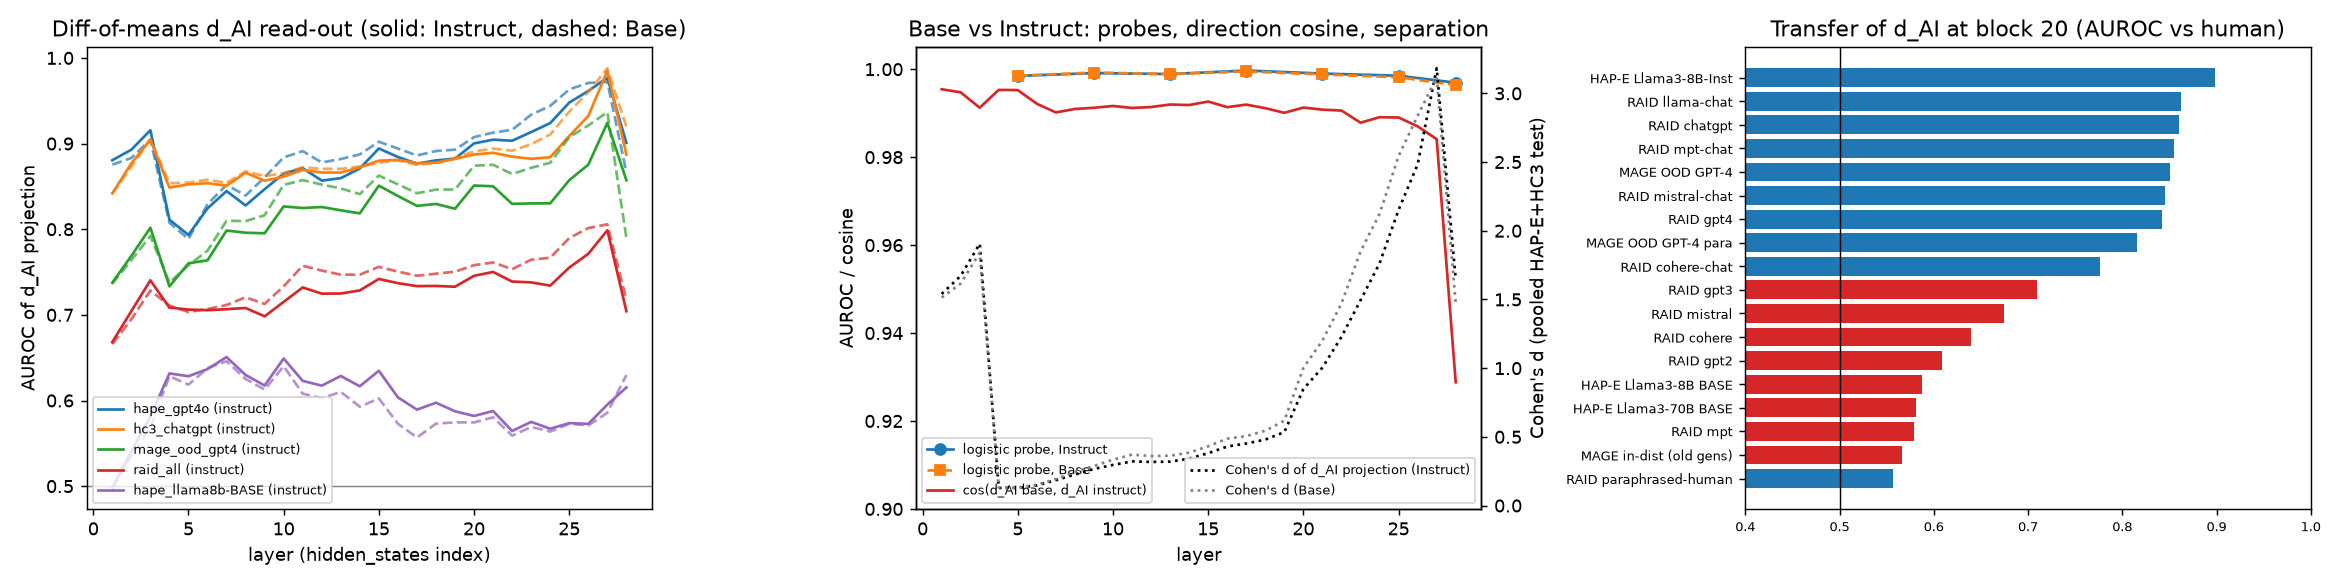
\includegraphics[width=0.99\linewidth]{figures/readout_layers_transfer.png}
    \caption{Read-out of \dai. \figleft{} AUROC of the \dai projection per layer for the instruct (solid) and base (dashed) models. Separation is good for chat generators but near chance for Llama-3-8B {\em base} continuations (purple). \figcenter{} Logistic probes reach 0.999 in both models, and $\cos(\daibase,\daiinst)$ stays $\ge 0.98$ at every layer. \figright{} Transfer at block 20: \dai separates chat and instruct generators (blue) from human text, but barely separates base and older LMs (red).}
    \label{fig:readout}
\end{figure}

\begin{table}[t]
    \centering
    \small
    \begin{tabular}{@{}lcc@{}}
        \toprule
        Test set (AUROC of \dai projection, block 20) & \textsc{Instruct} & \textsc{Base} \\
        \midrule
        \hape GPT-4o \versus human (same prefix) & 0.905 & {\bf 0.913} \\
        \hape Llama-3-8B-Instruct (unseen generator) & 0.899 & {\bf 0.909} \\
        \hcthree ChatGPT \versus human (same question) & 0.889 & {\bf 0.894} \\
        Fit \hape $\to$ test \hcthree / fit \hcthree $\to$ test \hape & 0.88 / 0.85 & 0.89 / 0.87 \\
        \mage OOD GPT-4 / GPT-4-paraphrased & 0.85 / 0.82 & 0.88 / 0.85 \\
        \raid chat generators (5) & 0.84--0.86 & 0.85--0.87 \\
        \midrule
        \raid base / older LMs (5) & 0.58--0.71 & 0.59--0.72 \\
        \hape Llama-3-8B / 70B {\em base} continuations & 0.59 / 0.58 & 0.58 / 0.58 \\
        \mage in-distribution (older generators) & 0.57 & 0.58 \\
        \raid paraphrased human \versus human & 0.56 & 0.55 \\
        \midrule
        Logistic probe, matched test (blocks 4--27) & 0.997--0.9997 & 0.996--0.9995 \\
        10 random directions (\hcthree, block 14) & 0.27--0.67 & -- \\
        \bottomrule
    \end{tabular}
    \caption{Read-out and transfer of \dai. A single direction separates content-matched pairs (AUROC $\approx$ 0.89--0.91) and transfers to unseen chat generators, but not to text from base LMs (bottom block). The base model's direction reads out equally well or slightly better.}
    \label{tab:readout}
\end{table}


{\bf Does a single direction separate human from AI text?} Yes. At block 20, the \dai projection reaches AUROC 0.89--0.91 on held-out content-matched pairs (\tabref{tab:readout}). It transfers across datasets (fitting on \hape and testing on \hcthree gives 0.88), to an unseen instruct generator (0.899), and to \raid and \mage chat generators (0.82--0.86).
It fails, however, on text from {\em base} language models: 0.58 on Llama-3 base continuations and 0.58--0.71 on older \raid generators (\figref{fig:readout}, right). A full logistic probe is near-perfect (0.997--0.9997), replicating \citet{quaremba2026linear}, but it uses many directions. We steer with the one-dimensional \dai because it is a cleaner object.
Random directions alone reach AUROCs between 0.27 and 0.67, because the residual stream is anisotropic, so moderate AUROCs ($\le 0.7$) for any single direction carry little meaning.

\subsection{Disentanglement: not formality, not the Assistant (H3)}
\label{sec:disentangle}

\begin{table}[t]
    \centering
    \small
    \begin{tabular}{@{}lccc@{}}
        \toprule
        Direction (block 20) & Raw cos with \dai & Whitened cos & AUROC (matched test) \\
        \midrule
        \dai & 1 & 1 & 0.869 \\
        \daiperp (6 confounds removed) & 0.78 & 0.26 & {\bf 0.970} \\
        \midrule
        Formality & $-0.23$ & 0.02 & 0.32 (0.68 flipped) \\
        Fluency (log-prob) & 0.06 & 0.05 & 0.51 \\
        Word length & 0.55 & $-0.01$ & 0.69 \\
        Domain (Reddit) & $-0.02$ & 0.01 & 0.51 \\
        Verbosity & 0.28 & 0.01 & 0.69 \\
        Assistant axis & 0.25 & {\bf 0.005} & 0.54 \\
        Post-training (Llama inst $-$ base) & {\bf 0.90} & 0.20 & 0.88 \\
        \midrule
        Null: random human/human split & $-0.09$ & 0.008 & 0.39 \\
        \bottomrule
    \end{tabular}
    \caption{Overlap of \dai with confound directions. In whitened geometry \dai is nearly orthogonal to every confound ($|\cos|\le 0.05$). The one large raw overlap is with an instruct-minus-base direction from Llama-3.}
    \label{tab:disentangle}
\end{table}


\Tabref{tab:disentangle} compares \dai with the confound directions. Raw cosines are misleading: word length (0.55), verbosity (0.28), and the Assistant axis (0.25) look related, but even a random split of human texts has raw cosine 0.44 with formality. After whitening, \dai is nearly orthogonal to every confound ($|\cos| \le 0.05$), including the Assistant axis (0.005).
Projecting the six-confound subspace out and refitting {\em raises} the difference-of-means AUROC from 0.89 to 0.98; the confounds added noise, not signal.
A cross-validated logistic regression on nine text covariates plus domain dummies reaches AUROC 0.944. The covariates are formality, log-probability, word length, length, contractions, an AI-ism lexicon, distinct-2, first person, and markdown. Adding the \dai projection raises this to 0.956. So \dai carries information beyond surface statistics, though it correlates moderately with some of them ($|r|\le 0.38$: longer words, fewer contractions, less first person).

{\bf What is \dai, then?} The one large overlap is with the {\em post-training} direction: Llama-3 instruct minus base continuations of the same prefix, from a different model family (raw cosine 0.90, whitened 0.20). Together with the transfer pattern in \secref{sec:readout}, this suggests that \dai encodes the style that instruction tuning produces, not ``machine-generated'' text in general.

\subsection{Causal steering (H2)}
\label{sec:steer}

\begin{figure}[t]
    \centering
    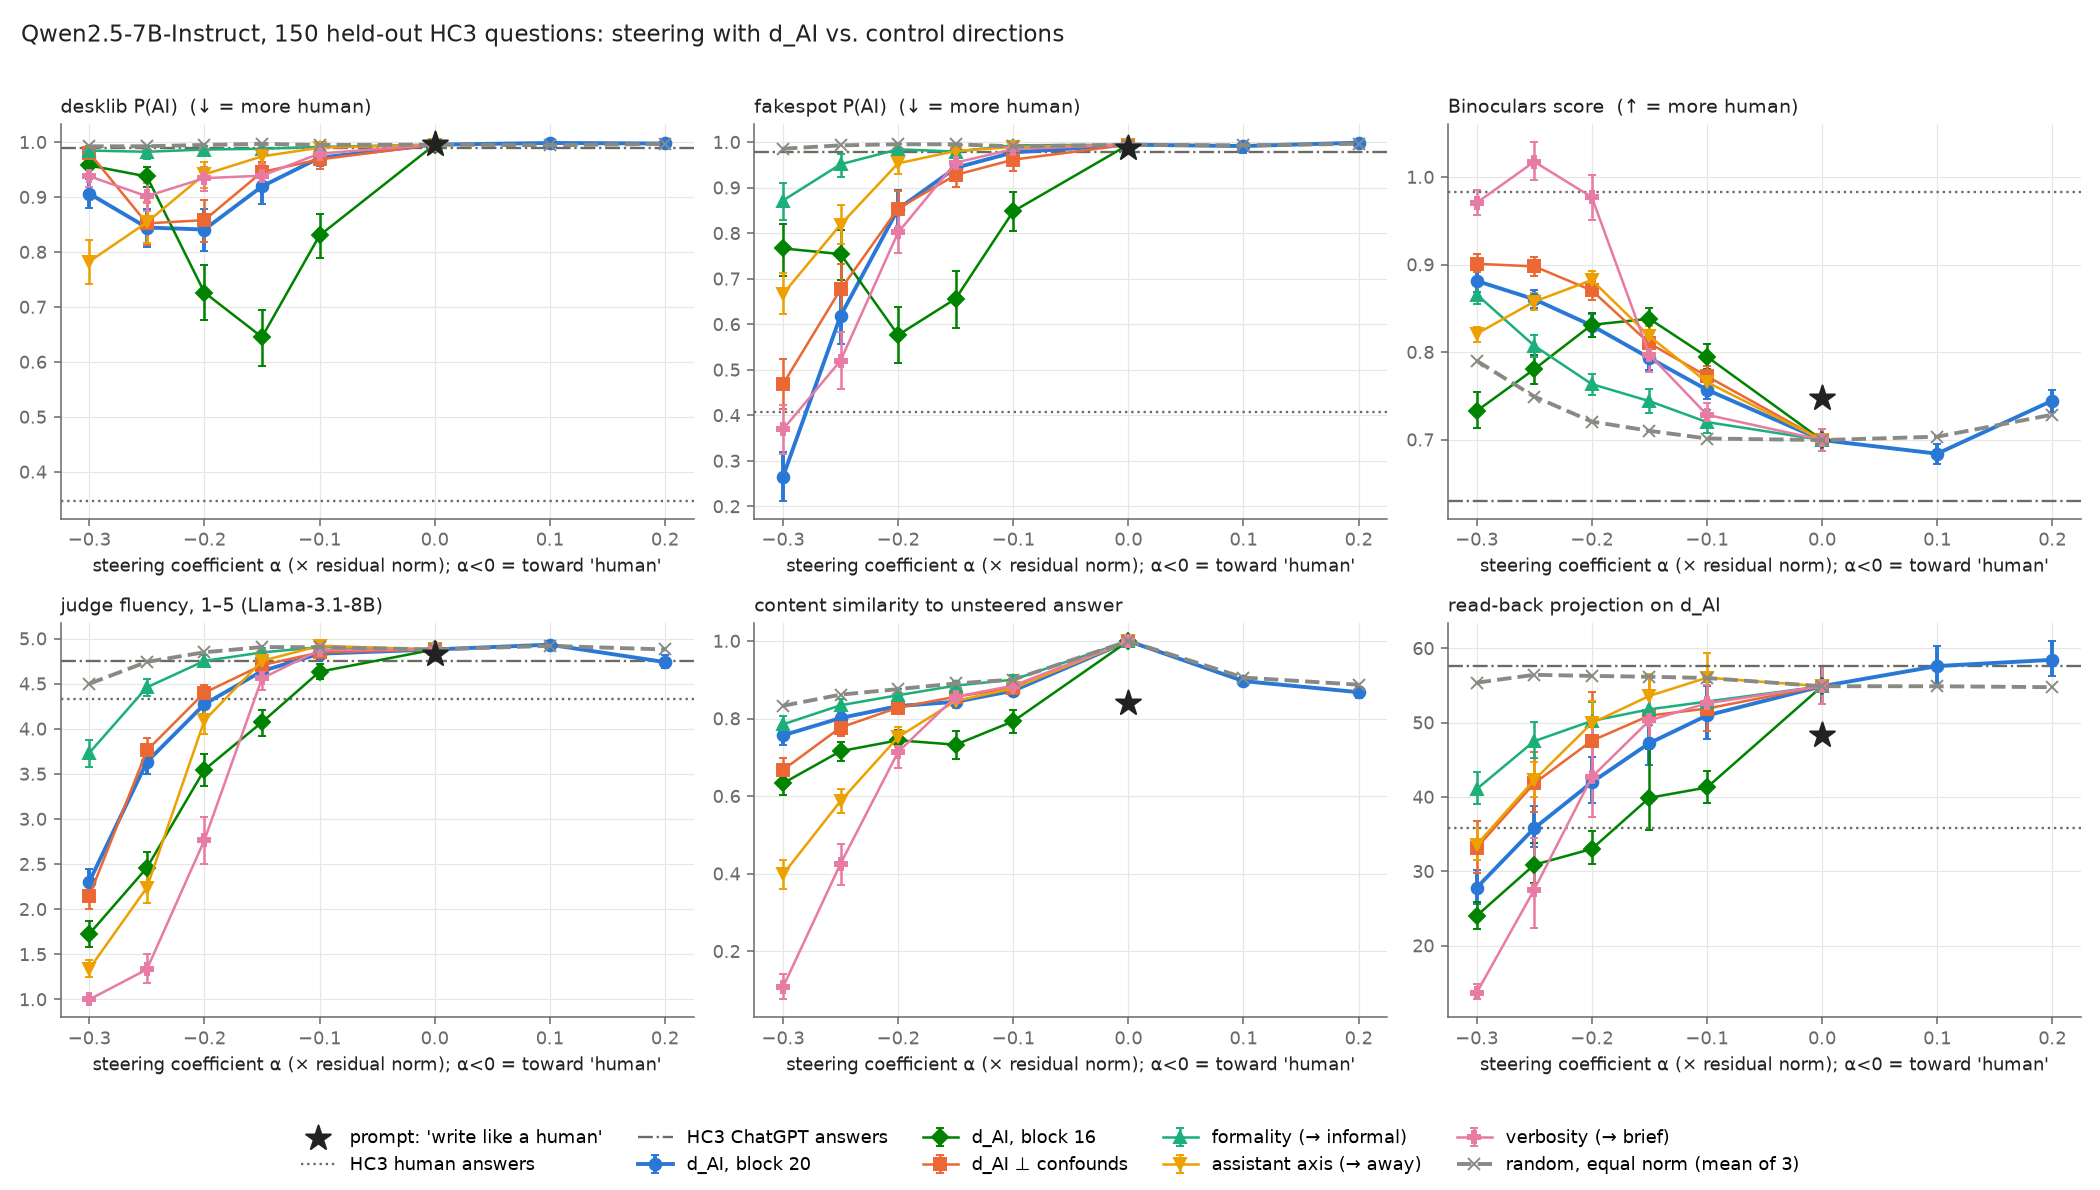
\includegraphics[width=0.99\linewidth]{figures/fig1_steer_dose_response.png}
    \caption{Dose--response of steering \qwen (150 held-out questions, 95\% CIs). {\em Top:} \dai at block 20 (blue), \daiperp (orange), and \dai at block 16 (dark green) lower the supervised detectors, while equal-norm random directions (gray) stay at ceiling. \binoculars rises for every perturbation, random included. {\em Bottom:} the cost in fluency, content similarity, and read-back projection. The ``write like a human'' prompt (star) leaves the supervised detectors untouched. Dotted and dash-dotted lines are \hcthree human and ChatGPT references.}
    \label{fig:dose}
\end{figure}

\begin{table}[t]
    \centering
    \resizebox{\textwidth}{!}{%
    \begin{tabular}{@{}lccccccc@{}}
        \toprule
        & \multicolumn{3}{c}{AI-ness} & \multicolumn{3}{c}{Coherence and content} & \\
        \cmidrule(lr){2-4} \cmidrule(lr){5-7}
        Condition & \desklib $\downarrow$ & \fakespot $\downarrow$ & \binoculars $\uparrow$ & Fluency & Relevance & Sim.\ to unsteered & Read-back \\
        \midrule
        Unsteered & 0.996 & 0.994 & 0.700 & 4.88 & 4.89 & 1.00 & 54.9 \\
        \midrule
        \dai $\alpha=-0.1$ & 0.972 & 0.978 & 0.757 & 4.83 & 4.89 & 0.87 & 51.0 \\
        \dai $\alpha=-0.15$ & 0.920 & 0.944 & 0.793 & 4.64 & 4.85 & 0.84 & 47.2 \\
        \dai $\alpha=-0.2$ & {\bf 0.841} & 0.853 & 0.830 & 4.27 & 4.72 & 0.83 & 42.0 \\
        \dai $\alpha=-0.25$ & 0.845 & 0.619 & 0.860 & 3.63 & 4.10 & 0.80 & 35.8 \\
        \dai $\alpha=-0.3$ & 0.906 & {\bf 0.266} & {\bf 0.881} & 2.31 & 2.52 & 0.76 & 27.8 \\
        \dai $\alpha=+0.2$ & 0.998 & 0.999 & 0.745 & 4.74 & 4.62 & 0.87 & 58.4 \\
        \daiperp $\alpha=-0.2$ & 0.858 & 0.854 & 0.871 & 4.40 & 4.61 & 0.83 & 47.6 \\
        Block-16 \dai $\alpha=-0.15$ & {\bf 0.645} & 0.656 & 0.838 & 4.07 & 4.33 & 0.73 & 39.9 \\
        \midrule
        Random (mean of 3) $\alpha=-0.2$ & 0.995 & 0.996 & 0.721 & 4.85 & 4.80 & 0.88 & 56.3 \\
        Random (mean of 3) $\alpha=-0.3$ & 0.993 & 0.986 & 0.790 & 4.50 & 4.53 & 0.83 & 55.4 \\
        Formality $\alpha=-0.25$ & 0.983 & 0.952 & 0.807 & 4.46 & 4.66 & 0.83 & 47.5 \\
        Formality $\alpha=-0.3$ & 0.985 & 0.872 & 0.866 & 3.73 & 4.00 & 0.79 & 41.1 \\
        Assistant axis $\alpha=-0.2$ & 0.941 & 0.954 & 0.882 & 4.09 & 3.57 & 0.75 & 49.9 \\
        Assistant axis $\alpha=-0.3$ & 0.783 & 0.667 & 0.821 & 1.34 & 1.02 & 0.40 & 33.6 \\
        Verbosity $\alpha=-0.15$ & 0.939 & 0.955 & 0.797 & 4.56 & 4.71 & 0.86 & 50.3 \\
        Prompt ``write like a human'' & 0.996 & 0.988 & 0.747 & 4.83 & 4.89 & 0.84 & 48.4 \\
        Prompt + \dai $\alpha=-0.15$ & 0.835 & 0.899 & 0.851 & 4.11 & 4.73 & 0.76 & 32.8 \\
        Zero-ablation of \dai (blocks 10--27) & 0.967 & 0.317 & 0.861 & 1.00 & 1.00 & 0.03 & 74.8 \\
        \midrule
        {\em \hcthree human answers} & {\em 0.348} & {\em 0.408} & {\em 0.982} & {\em 4.33} & {\em 4.26} & -- & {\em 35.8} \\
        {\em \hcthree ChatGPT answers} & {\em 0.990} & {\em 0.978} & {\em 0.630} & {\em 4.75} & {\em 4.83} & -- & {\em 57.6} \\
        \bottomrule
    \end{tabular}
    }
    \caption{Steering \qwen at block 20 (unless noted), means over 150 held-out questions. Negative $\alpha$ moves toward ``human''. Fluency and relevance are 1--5 judge scores (Llama-3.1-8B). Read-back is the unsteered model's projection of the output onto \dai. Best AI-ness values among steered conditions in {\bf bold}; note that the strongest values come with degraded fluency, so \figref{fig:matched} compares methods at matched coherence.}
    \label{tab:steer_main}
\end{table}


{\bf Does subtracting \dai make output read as more human?} Yes, on all three valid detectors. At block 20 and $\alpha=-0.2$, \desklib \pai falls from 0.996 to 0.841, \fakespot from 0.994 to 0.853, and \binoculars rises from 0.70 to 0.83 (\tabref{tab:steer_main}, \figref{fig:dose}).
Random directions of equal norm leave the supervised detectors at 0.99. Paired per prompt against the mean of three random directions, \dai lowers \desklib by $-0.154$ [$-0.20$, $-0.11$] ($p<10^{-10}$) and raises \binoculars by $+0.109$ at $\alpha=-0.2$. At $\alpha=-0.15$ the gaps are $-0.077$ and $+0.083$ (all $p<10^{-3}$).
The cost is a fluency drop from 4.88 to 4.27 at $\alpha=-0.2$ (\versus 4.85 for random). Relevance stays at 4.72, and similarity to the unsteered answer is 0.83 (\versus 0.88).
\daiperp, with all six confounds projected out, steers as well as \dai ($\desklib=0.858$ at $\alpha=-0.2$).
The ``write like a human'' prompt does not move \desklib at all (0.996).

\begin{figure}[t]
    \centering
    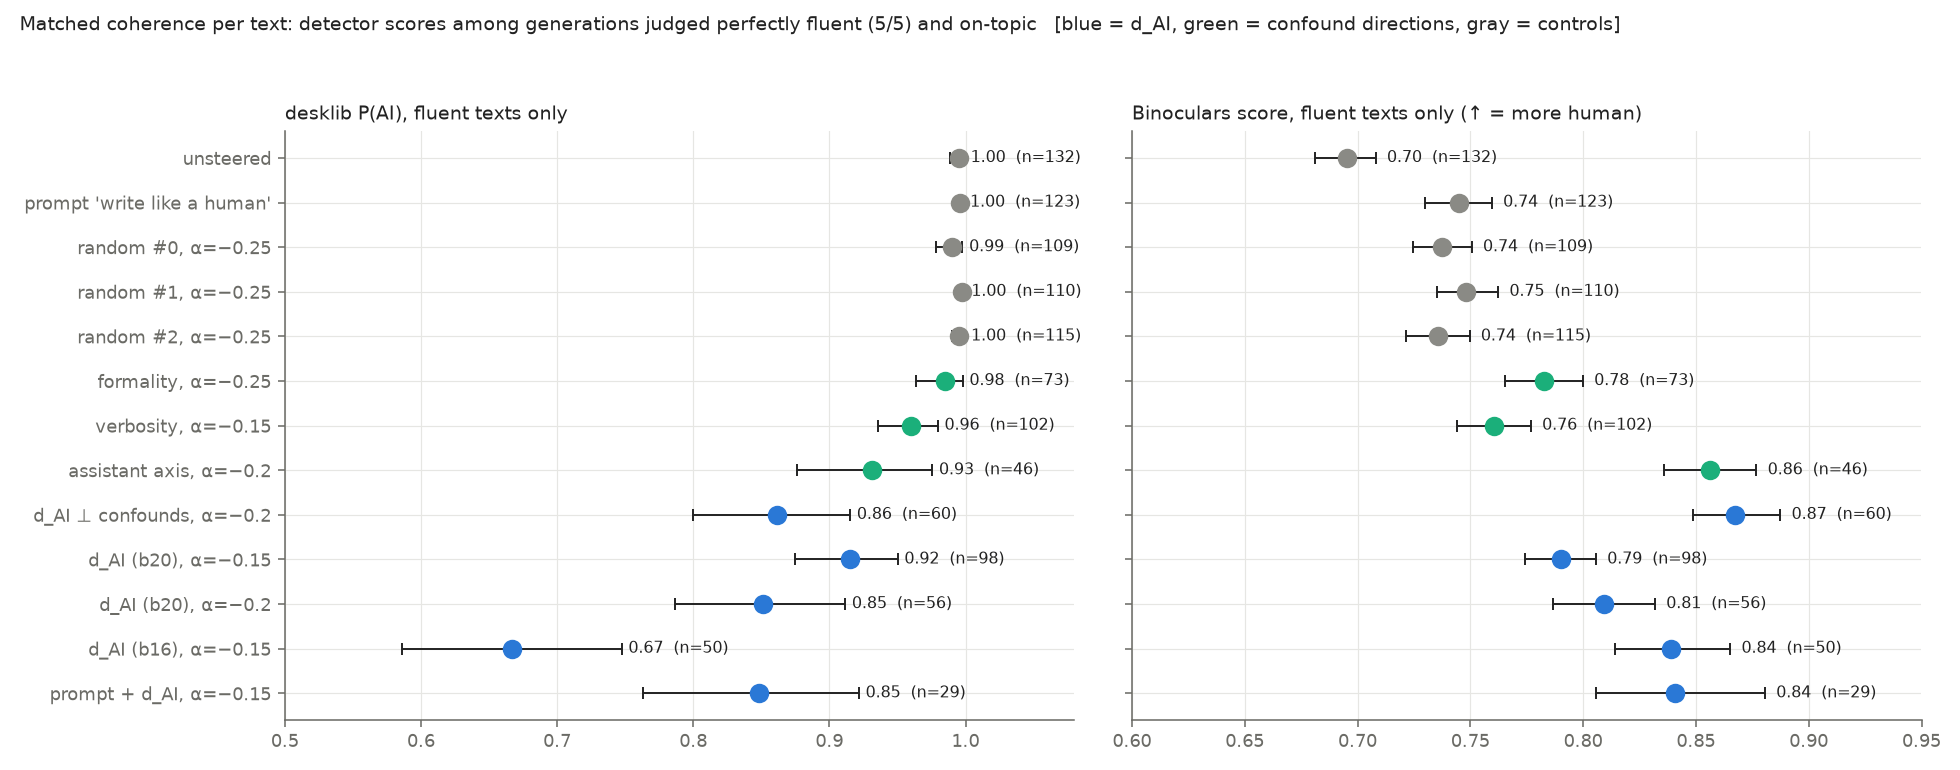
\includegraphics[width=0.99\linewidth]{figures/fig2_matched_coherence.png}
    \caption{Matched coherence per text. We keep only generations judged perfectly fluent (5/5), on-topic (relevance $\ge 4$), and in English. Among these, \dai and \daiperp (blue) still lower \desklib to 0.85--0.86 (0.67 at block 16), while random directions, the prompt (gray), and formality and verbosity (green) stay at 0.96--1.00. Error bars are 95\% bootstrap CIs; $n$ is the number of surviving texts.}
    \label{fig:matched}
\end{figure}

{\bf Is the effect just broken text?} No. \Figref{fig:matched} keeps only generations judged perfectly fluent and on-topic. In that subset, \dai at $\alpha=-0.2$ gives \desklib 0.85 ($n=56$) and \daiperp gives 0.86. Block-16 \dai gives 0.67, with 30\% of these fluent texts classified as human. By contrast, random directions give 0.99--1.00, formality 0.98, verbosity 0.96, the Assistant axis 0.93, and the prompt 1.00.
All \dai conditions differ from unsteered at $p<10^{-4}$ (Mann-Whitney); two of the three random directions do not differ significantly.
Per-condition matching agrees. We take the strongest $\alpha$ whose mean fluency and relevance stay within 0.5 of unsteered. \desklib is then 0.86 for \daiperp, 0.92 for \dai, 0.97 for the Assistant axis, 0.98 for formality, 0.99 for random, and 0.996 for the prompt.

{\bf Is \dai the Assistant persona?} No. Steering away from the Assistant axis lowers the detectors only once the text collapses: at $\alpha=-0.3$, \desklib is 0.78, but fluency is 1.34, relevance 1.02, and similarity to the unsteered answer 0.40. \dai moves the detectors while the answer and the assistant role stay intact.

\para{Binoculars is perplexity-confounded.} \binoculars rises under every perturbation, including random directions ($+0.09$ at $\alpha=-0.3$). Even among fluent texts, random steering moves it from 0.70 to 0.74, against 0.81 for \dai. The supervised detectors do not move under random steering, so we rely on them for the specificity claim.

\para{Positive steering.} Adding \dai cannot raise the supervised detectors, which are already at 0.996. It does raise the read-back projection to the ChatGPT-reference level (54.9 $\to$ 58.4) and, at $\alpha=+0.1$, lowers \binoculars to a more machine-like 0.68 ($p=0.001$). The base model, which is not at ceiling, shows the positive direction clearly (\secref{sec:base}).

\para{What changes in the text.} For the same prompt and seed, the unsteered answer opens ``{\em The forms 1099-MISC and K-1 serve different purposes in the tax system\ldots\ Let's break down each form: 1.\ **1099-MISC**: \ldots}''. At $\alpha=-0.25$ it becomes ``{\em I think you are mixing up two different things in taxation here: 1099-MISC and K-1. They are not to do with duplicate numbers, but are two differents tax forms\ldots}''.
Steering toward human adds first-person hedging, informal abbreviations, and small errors, while the answer keeps its topic and structure. Part of what detectors read as ``human'' is therefore {\em less polish}.

\para{Manipulation check.} At $\alpha=-0.25$, the unsteered model reads steered outputs exactly at the human level on \dai (read-back 35.8, equal to real human answers). Yet \desklib still gives 0.85, against 0.35 for human answers. Moving the model's own \dai coordinate to the human level captures only part of what external detectors respond to.

\subsection{In-distribution clamping: real but small}
\label{sec:clamp}

\begin{table}[t]
    \centering
    \resizebox{\textwidth}{!}{%
    \begin{tabular}{@{}lccccc@{}}
        \toprule
        Condition & \desklib & \fakespot & \binoculars & Fluency & Relevance \\
        \midrule
        \multicolumn{6}{@{}l}{\em Base model \qwenbase (Q/A completion format)} \\
        Unsteered & 0.938 & 0.772 & 0.740 & 4.66 & 4.18 \\
        Own \daibase $\alpha=-0.2$ & {\bf 0.870} & 0.693 & {\bf 0.818} & 4.31 & 3.63 \\
        Own \daibase $\alpha=+0.3$ & 0.959 & {\bf 0.914} & {\bf 0.670} & 4.69 & 4.49 \\
        Instruct \daiinst $\alpha=-0.2$ / $+0.3$ & 0.870 / 0.957 & 0.699 / 0.916 & 0.817 / 0.667 & 4.35 / 4.70 & 3.59 / 4.57 \\
        Random $\alpha=-0.2$ / $+0.3$ & 0.940 / 0.903 & 0.792 / 0.786 & 0.759 / 0.745 & 4.68 / 4.62 & 4.19 / 4.05 \\
        \midrule
        \multicolumn{6}{@{}l}{\em Instruct model \qwen, mean-clamp of the \dai coordinate} \\
        Unsteered & 0.996 & -- & 0.700 & 4.88 & -- \\
        Clamp b20 $\to$ AI mean & 0.997 & -- & 0.701 & 4.89 & -- \\
        Clamp b20 $\to$ human mean & 0.988 & -- & 0.727 & 4.89 & -- \\
        Clamp b20 $\to$ human mean $-$ 1 s.d. & {\bf 0.960} & -- & {\bf 0.757} & 4.82 & -- \\
        Clamp b10--27 $\to$ human mean & 0.967 & -- & 0.749 & 4.79 & -- \\
        Random directions, same clamp (3) & 0.994--0.996 & -- & 0.698--0.704 & 4.91--4.93 & -- \\
        \bottomrule
    \end{tabular}
    }
    \caption{{\em Top:} in the base model, \dai is causal in both directions, and the instruct model's direction works identically; random directions have no significant effect. Bold marks the strongest effect in each direction. {\em Bottom:} in-distribution clamping of the \dai coordinate in the instruct model gives small but direction-specific shifts with no fluency cost.}
    \label{tab:base_clamp}
\end{table}


Zero-ablating \dai destroys the text (fluency 1.00), because the human mean projection is not zero (32 at block 20). We therefore clamp the coordinate within its natural range instead (\tabref{tab:base_clamp}, bottom; \figref{fig:base}, right).
Clamping to the AI mean does nothing, since generations already sit there (54.9 \versus 53.6), which serves as a consistency check. Clamping to the human mean minus one standard deviation lowers \desklib to 0.960 and raises \binoculars to 0.757, with no fluency cost. Against the same clamp on random directions, the differences are $-0.034$ [$-0.052$, $-0.020$] for \desklib and $+0.057$ for \binoculars (both $p_{\text{holm}}<10^{-4}$).
The effect is specific but small. For scale, additive steering at $\alpha=-0.2$ shifts the coordinate by 71 units, about $3.3\times$ the natural human--AI gap of 21 units. Large detector effects need extrapolation beyond the range that human text occupies.

\subsection{Base \versus instruct: present before chat tuning (H4)}
\label{sec:base}

\begin{figure}[t]
    \centering
    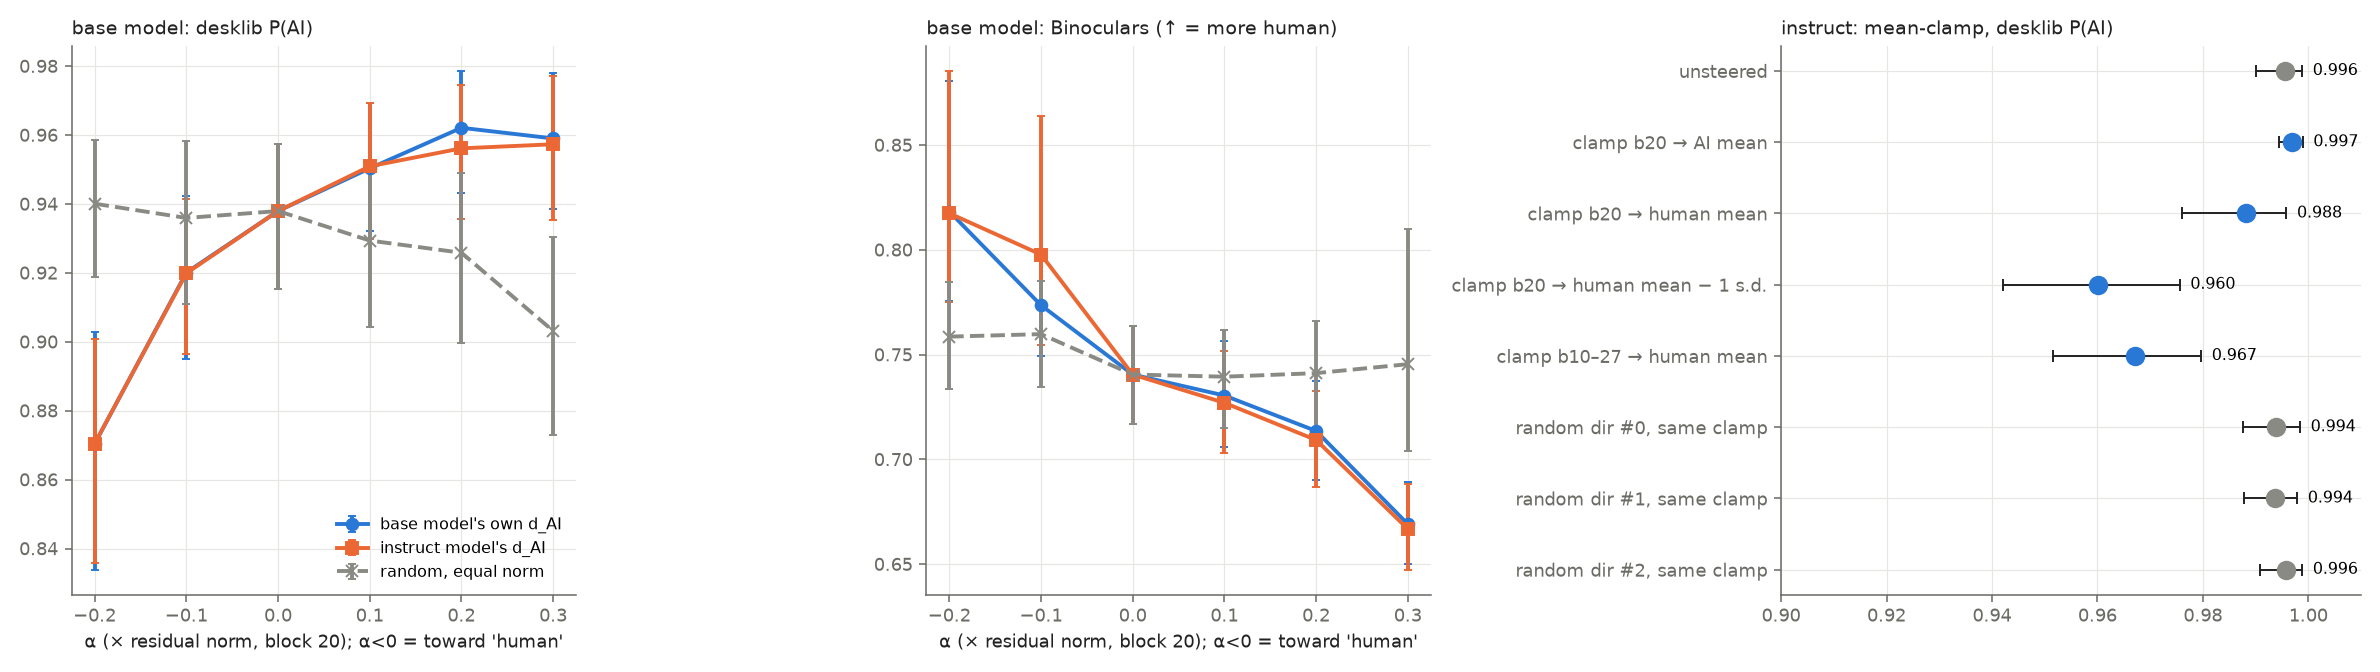
\includegraphics[width=0.99\linewidth]{figures/fig3_base_and_clamp.png}
    \caption{\figleft{} and \figcenter{} Steering the base model \qwenbase. Its own \dai (blue) and the instruct model's \dai (orange) give identical, bidirectional effects on \desklib and \binoculars, while a random direction (gray) is flat. \figright{} In-distribution mean-clamp in the instruct model. Clamping the \dai coordinate toward the human range gives small but direction-specific drops in \desklib; the same clamp on random directions has no effect.}
    \label{fig:base}
\end{figure}

The base and instruct directions are nearly identical: $\cos(\daibase,\daiinst)$ ranges from 0.984 to 0.995 across layers (0.991 at block 20). Base-model read-out is as good or slightly better (\tabref{tab:readout}; Cohen's $d$ 1.20 \versus 1.00 at block 20). Chat tuning neither creates nor sharpens the read-out direction.

In the base model, steering works in {\em both} directions (\tabref{tab:base_clamp}, top; \figref{fig:base}). Subtracting \daibase at $\alpha=-0.2$ lowers \desklib from 0.938 to 0.870 ($p_{\text{holm}}=8\times10^{-4}$) and raises \binoculars to 0.818. Adding it at $\alpha=+0.3$ raises \fakespot from 0.77 to 0.91 and lowers \binoculars to 0.670, while slightly {\em raising} relevance (4.18 $\to$ 4.49) and lengthening answers from 81 to 99 words. The instruct model's direction has the same effect, and random directions have no significant effect.
Base \qwenbase answers already look AI-like (\desklib 0.94; read-back 57.7, close to the ChatGPT references), consistent with a pretraining corpus that contains much synthetic and instruction-style data. Chat tuning moves the model's outputs further along the direction (\desklib 0.94 $\to$ 0.996, $p<10^{-4}$) without changing the direction itself.

\subsection{LLM judges: same sign, different ranking}
\label{sec:judges}

\begin{table}[t]
    \centering
    \resizebox{\textwidth}{!}{%
    \begin{tabular}{@{}lccccc@{}}
        \toprule
        Condition & AI-likelihood & $\Delta$ \versus unsteered [95\% CI] & $p_{\text{holm}}$ & Fluency & \% rated $<50$ \\
        \midrule
        Unsteered & 73.9 & -- & -- & 4.26 & 2\% \\
        \dai $\alpha=-0.15$ & 67.4 & $-6.2$ [$-10.7$, $-2.1$] & 0.038 & 4.06 & 8\% \\
        \dai $\alpha=-0.2$ & 67.7 & $-6.2$ [$-9.6$, $-3.0$] & 0.038 & 3.56 & 4\% \\
        \dai $\alpha=-0.25$ & 63.0 & $-10.9$ [$-17.5$, $-4.7$] & 0.061 & 2.64 & 20\% \\
        \daiperp $\alpha=-0.2$ & 68.5 & $-5.4$ [$-9.3$, $-1.9$] & 0.092 & 3.88 & 6\% \\
        Formality $\alpha=-0.25$ & 65.6 & {\bf $-$8.3} [$-11.7$, $-4.9$] & 0.001 & 3.70 & 8\% \\
        Assistant axis $\alpha=-0.2$ & 71.9 & $-2.0$ & 1.0 & 3.32 & 6\% \\
        Random 0/1/2 $\alpha=-0.2$ & 73.2/70.4/71.7 & $-0.7$/$-3.5$/$-2.2$ & $\ge 0.37$ & 4.18--4.20 & 0--2\% \\
        Prompt ``write like a human'' & 67.2 & $-6.7$ [$-9.8$, $-3.6$] & 0.004 & {\bf 4.24} & 6\% \\
        \dai $\alpha=+0.2$ & 75.3 & $+1.4$ & 1.0 & 3.94 & 0\% \\
        \midrule
        {\em \hcthree human answers} & {\em 54.5} & & & {\em 3.58} & {\em 38\%} \\
        {\em \hcthree ChatGPT answers} & {\em 69.8} & & & {\em 4.04} & {\em 0\%} \\
        \bottomrule
    \end{tabular}
    }
    \caption{Blind Cohere command-a-plus judge (0--100 AI-likelihood; 50 prompts per condition; Holm over 22 tests). The judge sees \dai lower AI-likelihood more than random directions do, but formality steering and prompting do at least as well. The judge itself is only weakly valid (AUROC 0.71).}
    \label{tab:cohere}
\end{table}


The blind Cohere judge agrees on the sign (\tabref{tab:cohere}). \dai at $\alpha=-0.2$ lowers AI-likelihood by 6.2 points relative to unsteered, and by 4.1 [$-7.0$, $-1.0$] relative to the mean of the random directions ($p=0.005$). A partial Nemotron-3-Super run at $\alpha=-0.1$ ($n\approx150$ per condition) agrees: \dai minus random is $-4.0$ [$-7.2$, $-0.9$] ($p=0.03$).
On these judges, however, \dai is {\em not} specific. Formality steering ($-8.3$) and the ``write like a human'' prompt ($-6.7$, with no fluency cost) do as well or better. On Nemotron, formality, the Assistant axis, and \daiperp score 69.6--69.9, similar to \dai's 70.1.
The judges appear to respond to surface register (informality, contractions, no markdown), which formality steering and prompting change directly. The supervised detectors rank the methods the other way round: \dai is far ahead, and formality, prompting, and random are similar. This is a real split between measures, not noise. Different readers of ``AI-ness'' key on different features, and \dai targets the one the trained detectors use.

\section{Discussion}
\label{sec:discussion}

{\bf Is there a ``sounds like AI'' direction?} There is a direction that the model reads out of text and also uses when writing. External detectors with other architectures recognise its effect. And it is specific: random, formality, verbosity, and Assistant-axis directions of equal norm do not reproduce its effect at matched coherence. Three qualifications shape what this direction is.

\para{It is chat-tuned style, not machine-ness.} \dai does not separate base-LM text from human text (AUROC 0.58). It nearly coincides with an instruct-minus-base direction from a different model family (raw cosine 0.90). This agrees with \citet{reinhart2024hape}, who find base Llama-3 close to human style, and with the failure of SV-Detect on base-model generators~\citep{vishnyakov2026svdetect}. What detectors and the direction share is the register that instruction tuning induces. That register is nonetheless already present in the pretrained \qwenbase, whose own answers score 0.94 on \desklib.

\para{It is not the Assistant persona.} The whitened cosine with the Assistant axis is 0.005. The raw cosine of 0.25 is at the level that anisotropy alone produces. Steering away from the Assistant changes detector scores only once the text degenerates, whereas \dai moves them while the answer and role stay intact. \citet{lu2026assistant} find the Assistant axis in base models, and we find the same for \dai. Both directions predate chat tuning, but they are different directions: ``sounding like AI'' and ``being the Assistant'' are separable in this model.

\para{It is a weak lever.} At the best coherent operating points, \desklib falls from 0.996 to 0.85--0.92 at block 20 or 0.67 at block 16. Human answers sit at 0.35, and only 5--30\% of fluent steered outputs flip to ``human''. The unsteered model reads steered text as human-level on \dai while the detectors do not. A full probe reaches 0.999 against 0.87 for the single direction, and the covariate model reaches 0.94. Together, these numbers show that AI-ness, as detectors see it, is multi-dimensional. This is a partial negative result for the ``single steerable feature'' reading.

{\bf Does the model write with what it reads?} Partly, and with low gain. In-distribution moves give statistically clear but tiny effects (\desklib $-0.03$ \versus random). Useful shifts require about $3\times$ extrapolation beyond the natural human--AI gap, where fluency begins to suffer. This matches reports that steering is weak on instruct models~\citep{steerweak2026} and trades off against quality~\citep{wu2025axbench}.

{\bf Prompting or steering?} The ``write like a human'' prompt changes surface features: the formality score drops from 0.84 to 0.60, markdown from 4.4 to 0.8 per 100 words, and contractions increase. Yet it does not fool the supervised detectors (0.996). Steering leaves markdown largely intact and still moves them. The detectors therefore key on something other than the formatting a prompt removes, and \dai reaches part of it. The two combine: prompt plus \dai gives the lowest read-back projection (32.8) and the highest flip rate (12\%). Unlike AxBench~\citep{wu2025axbench}, where prompting dominates, here the answer depends on the reader. Prompting wins on the LLM judge, and steering wins on trained detectors.

\para{Measure validity.} Our study shows how easily AI-ness measures can mislead. A local 8B judge is at chance on real human \versus ChatGPT answers, and \binoculars rises under random perturbations because steering raises perplexity. Only the supervised detectors are both valid (AUROC $\ge 0.98$) and stable under random perturbations. We encourage steering studies of style to report validity on reference texts and random-direction controls for every measure.

\para{Broader impact.} A direction that lowers detector scores could be used to evade detection. Our results show that this is not yet practical with one direction: outputs stay far from human-level scores, and fluency drops. They also show that supervised detectors depend partly on one linear feature that generators share, so detectors trained on chat-model text may fail on models whose post-training shifts that feature.

\subsection{Limitations}
\label{sec:limitations}
\begin{itemize}[leftmargin=*,itemsep=0pt,topsep=0pt]
    \item {\bf One model family.} We study only \qwen and \qwenbase, with block 20 as the primary layer and block 16 as the secondary layer, both chosen on a pilot. We did not run a Gemma-2 replication or an SAE analysis.
    \item {\bf Prompts and references.} The steering prompts are ELI5-heavy \hcthree questions in 5 domains, so the human references are Reddit and expert answers. Detectors score 120-word truncations.
    \item {\bf Detectors.} The training data of \desklib and \fakespot is undocumented and may overlap \hcthree, although neither saw our steered outputs or activations. \binoculars is perplexity-confounded. The Cohere judge covers 50 prompts $\times$ 14 conditions, and Nemotron covers only $\alpha=-0.1$ because of API limits.
    \item {\bf Coherence.} Coherence is judged by an 8B model. Its ratings are plausible (gibberish scores 1, references 4.3--4.8) but coarse. Content drifts somewhat (similarity 0.83 for \dai \versus 0.88 for random at $\alpha=-0.2$). We ran no human evaluation.
    \item {\bf Assistant axis.} Ours is a cheap rebuild (40 roles $\times$ 20 questions) rather than the full PCA axis of \citet{lu2026assistant}. The Assistant and verbosity directions also come from chat-context activations, whereas \dai comes from raw text. Some of the near-zero whitened cosine may reflect this difference in context.
    \item {\bf Ceilings and seeds.} Detector ceilings hide positive-direction effects in the instruct model. We use a single seed per prompt, with the 150 prompts as the unit of replication.
\end{itemize}

\section{Conclusion}
\label{sec:conclusion}

We asked whether the human-\versus-AI direction that detectors read from the residual stream also controls how AI-like a model's writing sounds. In \qwen it does.
Subtracting \dai lowers supervised detector scores (\desklib 0.996 $\to$ 0.84) and raises the zero-shot \binoculars score. Equal-norm random directions, formality, verbosity, the Assistant axis, and a ``write like a human'' prompt fail to match this at equal coherence, and the effect holds among perfectly fluent outputs and after projecting out six confounds.
The direction is better described as the style signature of chat tuning than as ``machine text''. It is distinct from the Assistant persona, and it already exists, with the same orientation, in the base model, which it steers in both directions.
It is also a weak lever. Fluent steered text remains far from human scores, in-distribution clamping barely moves detectors, and an LLM judge finds prompting equally effective.

{\bf Takeaway:} ``sounding like AI'' has a real, causal linear component, but no single direction captures it.

\para{Future work.} We plan to steer with a low-rank subspace of the human--AI difference instead of one vector, and to apply steering only after the first sentence. We also plan to replicate on Gemma-2 with SAE features and on Llama-3.1-8B, to run human evaluation of fluent steered outputs, and to test whether the detectors' remaining signal lives in formatting by combining \dai with markdown removal.


\bibliography{references}

\appendix
\section{Reproducibility Details}
\label{app:details}

\para{Implementation.} We use Python 3.12, PyTorch and Transformers in bf16, scikit-learn, and sentence-transformers. Directions are fit with seed 0, and generation uses seed 1234 for every condition batch.

\para{Pipeline.} Data construction, activation extraction (raw text, mean-pooled, all layers, both models), covariate scoring, confound generation, direction fitting with read-out (E1), disentanglement (E2), steering generation for the instruct model, mean-clamp and base model (E3, E3b, E4), detector scoring, read-back projection, LLM judging, and analysis are separate scripts. They are run in that order.

\para{Compute.} All experiments run on one NVIDIA RTX A6000 (48\,GB). Activation extraction takes about 15 minutes. Generation takes about 25 seconds per 150-prompt condition, or about 30 minutes for the main run. Detectors and \binoculars take about 25 minutes per 9,000 texts, and the local judge about 15 minutes. API judges used free tiers (about 700 Cohere and 1,035 OpenRouter calls).

\para{Judge prompt.} Each judge sees one answer and its question, without the condition. It returns a 0--100 probability that the answer was written by an AI, a 1--5 fluency score, and a 1--5 relevance score. The local judge decodes greedily.

\para{Layer and scale selection.} On 30 pilot questions disjoint from the 150 test questions, we steered at several layers and coefficients before running the main experiment. Block 20 kept output in English and preserved content best. Text collapsed for $|\alpha|>0.3$, so the main grid spans $\alpha\in[-0.3,-0.1]$ with $\|\bar\vh\|=355.7$.


\end{document}
